\documentclass[12pt]{article}
\usepackage{amssymb,amsmath,times}
\usepackage{color}
\usepackage{graphicx}
\usepackage{fancyhdr}
\usepackage{multirow}
\usepackage{cite}
\usepackage{color}
\usepackage{natbib}

% define formatting
%\pagestyle{empty}
\parindent=0pt
\topmargin=0.in \headheight=0in \headsep=-0.1in \textheight=9.2in
\textwidth=6.5in \oddsidemargin=0in

\def\Neff{{N_{\rm eff}}}


% define spacings
\def\p{\smallskip}
\def\sp{\vspace{0.15in}}
\def\spa{\vspace{0.3in}}
\def\spaa{\vspace{0.5in}}
\def\spaaa{\vspace{0.7in}}

% define shorthands for latex commands
\def\bei{\begin{itemize}}
\def\eei{\end{itemize}}

% define commonly used symbols
\def\et{{\it et al.\ }}
\def\degr{$^{\circ}$}
\def\arcsec{$^{\prime\prime}$}
\def\pp{\pi}

% define various names
\def\usk{ }
\def\max{MAX}
\def\maxima{MAXIMA}
\def\boom{BOOMERanG}
\def\arch{Archeops}
\def\maxboom{\maxima/\boom}
\def\planck{Planck}
\def\combat{COMBAT}
\def\cmb{CMB}
\def\cmba{CMBA}
\def\tic{Ticra}
\def\codef{CODE5}
\def\forecast{FORECAST}
\def\maxipol{MAXIPOL}
\def\hwp{HWP}
\def\ahwp{AHWP}
\def\wmap{WMAP}
\def\igb{IGB}
\def\apex{APEX}
\def\ebex{EBEX}
\def\squid{SQUID}
\def\ld{LD}
\def\ldii{LD-II}
\def\blast{BLAST}
\def\pb{\sc polarbear}
\def\pbsa{{\sc polarbear}/SA}
\def\spttg{SPT3G}
\def\ebextw{EBEX2013}
\def\ebexsk{EBEX-IDS}
\def\litebird{LiteBIRD}
\def\bicep{BKA}
\def\biceptwo{BICEP2}
\def\dfmux{DFMux}
\def\xsixf{$\times$64}
\def\xones{$\times$16}

%define physics and cosmological notations
\def\het{$^{3}$He}
\def\hef{$^{4}$He}
\def\lnt{lN$_{2}$}
\def\wn{cm$^{-1}$}
\def\omeg{$\Omega$}
\def\omegb{$\Omega_{b}$}
\def\hubble{$H_{0}$}
\def\lamb{$\Lambda$}
\def\cl{$C_{\ell}$}
\def\micron{$\mu$m}
\def\microk{$\mu{\mbox{K}}$}
\def\microkrtsec{$\mu{\mbox{K}}\sqrt{\mbox{sec}}$}
\def\microkprthz{$\mu{\mbox{K}}/\sqrt{\mbox{Hz}}$}
\def\wattrthz{${\mbox{Watt}}\sqrt{\mbox{Hz}}$}
\def\voltprthz{${\mbox{Volt}}/\sqrt{\mbox{Hz}}$}
\def\sintheta{\mbox{$\sin\theta$}}
\def\bceti{$\beta$-ceti}
\def\etad{$\eta$-draconis}
\def\ruo2{RuO$_{2}$}
\def\tdot{$\dot{\theta}$}
\def\taub{$\tau_{b}$}
\def\degsq{deg$^2$}

% define polarization symbols parameters
\def\It{$I_{t}$}  
\def\sq{$Q$}
\def\su{$U$}
\def\dsu{$\Delta U$}
\def\dsq{$\Delta Q$}
\def\TT{$C_l^{\rm TT}$}
\def\TE{$C_l^{\rm TE}$}
\def\EE{$C_l^{\rm EE}$}
\def\BB{$C_l^{\rm BB}$}

% define math and vectors

\def\mathrelfun#1#2{\lower3.6pt\vbox{\baselineskip0pt\lineskip.9pt
  \ialign{$\mathsurround=0pt#1\hfil##\hfil$\crcr#2\crcr\sim\crcr}}}
\def\simlt{\mathrel{\mathpalette\mathrelfun <}}
\def\simgt{\mathrel{\mathpalette\mathrelfun >}}

\def\hatx{{\bf \hat n}}
\def\hatnprime{{\bf \hat n'}}
\def\hatnone{{\bf \hat n}_1}
\def\hatntwo{{\bf \hat n}_2}
\def\hatni{{\bf \hat n}_i}
\def\hatnj{{\bf \hat n}_j}
\def\vecx{{\bf x}}
\def\veck{{\bf k}}
\def\hatx{{\bf \hat x}}
\def\hatk{{\bf \hat k}}
\def\hatz{{\bf \hat z}}
\def\VEV#1{{\left\langle #1 \right\rangle}}
\def\cP{{\cal P}}
\def\noise{{\rm noise}}
\def\pix{{\rm pix}}
\def\map{{\rm map}}
\long\def\comment#1{}

% \newcommand{\beq}{\begin{equation}}
% \newcommand{\eeq}{\end{equation}}
% \newcommand{\bea}{\begin{eqnarray}}
% \newcommand{\eea}{\end{eqnarray}}
\newcommand\PRL{{\it Phys.~Rev.~Lett.}}
\newcommand\prl{{\it Phys.~Rev.~Lett.}}
\newcommand\ApJ{{\it Ap.~J.}}
\newcommand\apj{{\it Ap.~J.}}
\newcommand\ApJL{{\it Ap.~J.~Lett.}}
\newcommand\apjl{{\it Ap.~J.~Lett.}}
\newcommand\ApJS{{\it Ap.~J.~Suppl.}}
\newcommand\apjs{{\it Ap.~J.~Suppl.}}
\newcommand\PR{{\it Phys.~Rev.}}
\newcommand\PL{{\it Phys.~Lett.}}
\newcommand\MNRAS{{\it MNRAS}}
\newcommand\mnras{{\it MNRAS}}
\newcommand\MNRASL{{\it MNRAS\ Lett.}}
\newcommand\AnA{{\it Astron.~Astrophys.}}
\newcommand\BAAS{{\it Bull.~Am.~Astron.~Soc.}}
\newcommand\NP{{\it Nucl.~Phys.}}
\newcommand\RMP{{\it Rev.~Mod.~Phys.}}
\newcommand\ARAA{{\it ARAA}}
\newcommand\prd{{\it Phys.~Rev.~D.}}
\newcommand\plb{{\it Phys.~Lett.~B.}}
\newcommand\ao{{\it Appl.~Optics}}
\newcommand\aap{{\it Astron.~Astrophys.}}
\newcommand\aaps{{\it Astron.~Astrophys.~Suppl.}}
\newcommand\pasp{{\it Proc.~Ast.~Soc.~Pac.}}
\newcommand\josa{{\it J.~Opt.~Soc.~Am.}}
\newcommand\phr{{\it Phys. Reports}}
\newcommand\aj{{\it Astronomical Journal}}
\newcommand\jcap{{\it JCAP}}
\newcommand\apss{{\it ApSS}}

\newcommand{\comred}[1]{\textcolor{red}{#1}}

% Let's you define a command for both text and math mode. 
\newcommand{\wisk}[1]{{\ifmmode{#1}\else{$#1$}\fi}}



\setlength{\floatsep}{0.5\floatsep}
\setlength{\textfloatsep}{0.5\textfloatsep}
\setlength{\intextsep}{0.5\intextsep}
\setlength{\floatsep}{0.5\floatsep}
\setlength{\dblfloatsep}{0.5\dblfloatsep}
\setlength{\dbltextfloatsep}{0.5\dbltextfloatsep}

\begin{document}

\bibliographystyle{unsrt}

\setlength{\baselineskip}{1.0\baselineskip}
\setlength{\parskip}{1.\parskip}

\parindent = 15pt

\tableofcontents

\setcounter{figure}{0}

\newpage
%\twocolumn

\section{Scientific, Technical, and Management Section}



\vspace{-0.13in}

\comred{0.5 pg. executive summary goes here.}

Shaul is writing this. Due by Nov. 4.


\vspace{-0.22in}


\subsection{Baselines and Observables}
\label{sec:observables}

\vspace{-0.05in}

We are proposing to study a probe-scale mission to extract the wealth 
of cosmological information contained in the spectrum and polarization of the \ac{CMB}. 
The starting points for our study of this CMB Probe are two current-decade space missions, 
EPIC-IM and Super-PIXIE~\cite{bock2009, Kogut2011PIXIE}. EPIC-IM was presented 
to the 2010 decadal panel as a candidate \ac{CMB} imaging polarization space mission. 
It was based on a 2~m aperture telescope and 11,094 bolometric transition edge sensors. 
PIXIE is a proposed Explorer-scale mission focused on a measurement of the spectrum 
and polarization of the CMB on large angular scales. Super-PIXIE is envisioned to be a scaled up, 
more capable version of PIXIE. It consists of 4 spectrometers, each operating between 
30 and 6015~GHz with 400 15~GHz-wide bands. Improvements in technology by the next decade will enable 
the design of a mission that is more capable compared to EPIC-IM and Super-PIXIE. Therefore, all 
quantitative predictions presented in this proposal, which are based on EPIC-IM and Super-PIXIE, 
represent {\it minimum} capabilities for the CMB Probe. 

The best measurements of the \ac{CMB} spectrum -- made by COBE/FIRAS approximately 25 years ago --
show that the average CMB spectrum is consistent with that of a blackbody to an accuracy of 4 parts 
in $10^{4}$~\cite{Mather1994, Fixsen1996}. Distortions in this spectrum encode a wealth of new information.
The distortion shapes are commonly denoted as $\mu$- and $y$-types~\cite{Zeldovich1969, Sunyaev1970mu}. The 
$\mu$-distortion arises from energy release in the early Universe and can only be produced in the hot and dense 
environment present at high redshifts. This makes $\mu$-distortions a novel messenger from a redshift 
range $ z \geq 5\times10^{4} $. The $y$ distortions are caused by 
energy exchange between \ac{CMB} photons and free electrons through inverse Compton 
scattering. These originate at lower redshifts and are sensitive to the 
evolution of the large scale structure of the Universe. 

Thomson scattering at the surface of last scattering is the source of the polarization of the \ac{CMB}. It is useful 
to decompose the polarization field to two modes that are independent over the full sky, $E$ and $B$ modes. 
Together with the pattern of temperature anisotropy $T$, the \ac{CMB} thus gives three auto- and three cross-spectra. 
The {\it Planck} satellite and larger aperture ground-based instruments measured the $T$ spectrum to cosmic
variance limit for $\ell \leq ??$. Much information remains encoded in the $E$ and $B$ spectra, whose full exploration 
has just begun~\cite{planck,spt,polarbear,bicep}.   

A future \ac{CMB} Probe-scale mission will address the physics of the big bang and of quantum gravity; it will 
measure the sum of the neutrino masses, and constrain the effective number of light particle species and 
the nature of dark matter; it will probe the existence of new forms of matter at the early Universe; it will 
give new insights on the star-formation history across cosmic times, and it will provide information about 
the processes that control structure formation. In addressing these broad array of fundamental questions the 
Probe firmly fits into NASA's strategic plan as articulated by its Strategic Goal~1 ``Expand the frontiers of knowledge", 
and specifically Objective~1.6 ``Discover how the Universe works, [and] explore how it began and evolved".
%and three
%for the temperature ($T$) 
%and for the Scalar perturbations, 
%such as primordial energy density perturbations only give $E$-modes. The $B$-mode is a unique probe of early Universe 
%tensor perturbations, such as Inflation~\cite{kamionkowski97a,zaldarriaga97}. 

%\begin{table}[h]
%\small
%\centering
%%\begin{adjustbox}{width=1\textwidth,center}
%\begin{tabular}{|c|c|c|c|c|c|c|}
%\hline
%{\bf Freq} & { $\theta_{FWHM}$} & {\bf N$_{bol}^a$} & \multicolumn{2}{|c|}{\bf NET [$\pmb\mu$K $\sqrt{s}$]} & {\bf w$_p^{-1/2}$} & {\bf $\delta T_{pix}^e$ } \\ \cline{4-5}
%{\bf [GHz]} & {\bf [$'$]} & {\bf [\#]} & {\bf bolo$^b$} & {\bf band$^c$} & {\bf [$\mu$K-$'$]$^d$} & {\bf [nK]} \\ \hline
%30  & 28  & 84   & 84  & 9.2 & 14 & 83 \\ \hline
%45  & 19  & 364  & 71  & 3.7 & 5.7 & 34 \\ \hline
%70  & 12  & 1332 & 60  & 1.6 & 2.5 & 15 \\ \hline
%100 & 8.4 & 2196 & 54  & 1.1 & 1.8 & 10 \\ \hline
%150 & 5.6 & 3048 & 52  & 0.9 & 1.4 & 8  \\ \hline
%220 & 3.8 & 1296 & 59  & 1.6 & 2.5 & 15 \\ \hline
%340 & 2.5 & 744  & 100  & 3.7 & 5.6 & 33 \\ \hline
%500 & 1.7 & 1092 & 350  & 10  & 16 (140)$^f$ & 8$^g$ \\ \hline
%850 & 1.0 & 938  & 15000  & 280 & 740 (70)$^f$ & 7$^g$ \\ \hline
%{\bf Total$^h$} & & {\bf 11094} & & {\bf 0.6} & {\bf 0.9} & {\bf 5.4} \\
%\hline
%\multicolumn{3}{|l}{\footnotesize$^a$Two bolometers per focal plane pixel} & \multicolumn{4}{l|}{\footnotesize$^e$Sensitivity $\delta$T$_{CMB}$ in a $2^{\circ} \times 2^{\circ}$ pixel} \\
%\multicolumn{3}{|l}{\footnotesize$^b$Single bolometer sensitivity, CMB temperature} & \multicolumn{4}{l|}{\footnotesize$^f$Point source sensitivity in $\mu$Jy/beam (1$\sigma$) w/o confusion} \\
%\multicolumn{3}{|l}{\footnotesize$^c$Sensitivity combining all bolometers in a band} & \multicolumn{4}{l|}{\footnotesize$^g$Surface brightness sensitivity, Jy/sr, $2^{\circ} \times 2^{\circ}$ pixel (1$\sigma$) } \\
%\multicolumn{3}{|l}{\footnotesize$^d[8\pi \mbox{NET}_{bolo}^2 / (T_{mis}N_{bol})]^{1/2}(10800/\pi)$} & \multicolumn{4}{l|}{\footnotesize$^h$Combining all bands together} \\
%\hline
%\end{tabular}
%\end{adjustbox}
%\vspace{-0.13in}
%\caption{ \small \setlength{\baselineskip}{0.96\baselineskip}
%EPIC sensitivities. 
%\label{tab:epic} }
%\normalsize
%\vspace{-0.05in}
%\end{table}


%at a temperature 
%$T_0=(2.726\pm 0.001)\,{\rm K}$~\citep{Mather1994, Fixsen1996}. These are the best measurements
%of the average spectrum to date, 

%but next generation CMB spectrometers are expected to greatly improve the $\mu$-distortion limits of COBE/FIRAS \citep{Kogut2011PIXIE}. Several standard processes that encode unique information about the Universe are expected to {\it distort} the CMB spectrum \citep[e.g.,][]{Chluba2016LCDM} at a level that is within reach of present-day technology \citep{Kogut2011PIXIE, PRISM2013WPII}.  The classical distortion shapes, commonly denoted as $y$- and $\mu$-type distortions, arise from early energy release and subsequent energy exchange of CMB photons with free electrons through inverse Compton scattering \citep{Zeldovich1969, Sunyaev1970mu}. A $\mu$-distortion can only be produced in the hot and dense environment present at redshifts $z\gtrsim 5\times10^4$, while $y$-type distortions are caused at lower redshifts. This makes $\mu$-distortions a unique messenger from the early Universe. 




%In addition to the CMB temperature and polarization anisotropy targeted by CMB imagers, {\it unique} new information about 
%early-universe physics can be gained by studying the energy spectrum of the CMB~\citep{Sunyaev1970SPEC, Burigana1993, Hu1993, %Chluba2011therm}. 


\vspace{-0.22in}


\subsection{Science Objectives}
\label{sec:science}

\vspace{-0.05in}
 
\subsubsection{The Primordial Universe and Cosmic Inflation}

\vspace{-0.05in}

%The observed temperature and $E$-mode polarization of the \ac{CMB} imply the existence of primordial 
%density perturbations that were generated long before recombination, providing a remarkable 
%observational link to the dynamics of the universe near the big bang.
%In the context of general relativity, these primordial density perturbations can be generated causally 
%either during a contracting phase followed by a bounce or during inflation, a primordial era of 
%accelerated expansion.
%Inflation, a primordial era of accelerated expansion, provides a compelling dynamical origin for the observed nearly scale-invariant spectrum of these primordial perturbations~\cite{guth81,linde82,albrecht82,sato81,kolb94}. 
%Unlike observationally viable bouncing cosmologies, 
The simplest models of inflation, a primordial era of accelerated expansion, predict as yet unobserved primordial gravitational waves with a nearly scale-invariant spectrum, sourced directly by quantum fluctuations of the tensor component of the metric. 
%In addition to primordial density perturbations inflation predicts an as yet unobserved spectrum of primordial gravitational waves sourced directly by quantum fluctuations of the tensor component of the metric. 
These gravitational waves leave a distinct $B$-mode imprint on the polarization of the \ac{CMB}. Any 
detection of primordial $B$-mode polarization, whether generated by the gravitational waves 
of inflation~\cite{kamionkowski97a,zaldarriaga97} or any other source of vector or tensor perturbations, 
such as primordial magnetic fields \cite{Seshadri:2000ky,Lewis:2004ef,Ade:2015cao,Zucca:2016iur} and 
cosmic strings \cite{Turok:1997gj,Seljak:2006hi,Avgoustidis:2011ax,Moss:2014cra} would reveal completely 
new information about the early universe. The results would either provide additional confirmation for 
current models or could overturn them. A detection would also have implications for fundamental physics 
by providing evidence for a new energy scale near the GUT scale. For example, in single-field inflation 
the potential energy density $V$ of the inflaton is related to the tensor-to-scalar ratio $r$ by 
$V^{1/4} = 3.3 \times 10^{16} \ r^{1/4}\,\, {\rm GeV}$. 

%Figure~\ref{fig:clall} shows current CMB data, $B$ modes from vacuum fluctuations of the metric during an inflationary era for two representative values of $r$, as well as forecasts for the determination of the \ac{CMB} spectra for EPIC-IM. 
To test inflation, the largest scales $\ell \leq 10$ are particularly important because they may reveal 
the presence of $B$-mode correlations on scales that were super-horizon at the time of 
recombination~\cite{Lee:2014cya}, 
and because on large scales the signal is strongest relative to the lensing $B$ mode and instrumental 
noise.
In its recent report New Worlds New Horizons (NWNH), the decadal survey committee strongly endorsed 
searches for $B$ modes from inflation saying, ``The convincing detection of $B$-mode polarization in 
the CMB produced in the epoch of reionization would represent a watershed discovery.''~\cite{blandford2010}. 
 Figure~\ref{fig:clall} shows current CMB data, $B$ modes from vacuum fluctuations of the metric 
%during an inflationary era 
for two representative values of $r$, forecasts for the determination 
of the \ac{CMB} spectra for EPIC-IM as well as the lensing residual and noise.
No sub-orbital platform has yet produced measurements of $B$ modes at $\ell< 40$, and a satellite is by 
far the most suitable platform for the all-sky observations necessary to reach the lowest modes, $\ell<20$. 
\begin{figure}[ht!]
\begin{center}
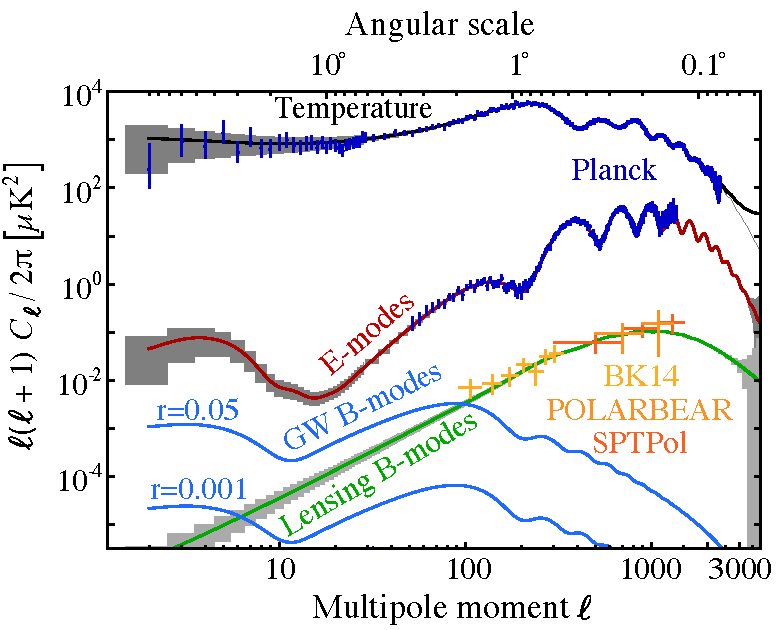
\includegraphics[width=3in]{figs/cmb_powspec_v1.pdf}  
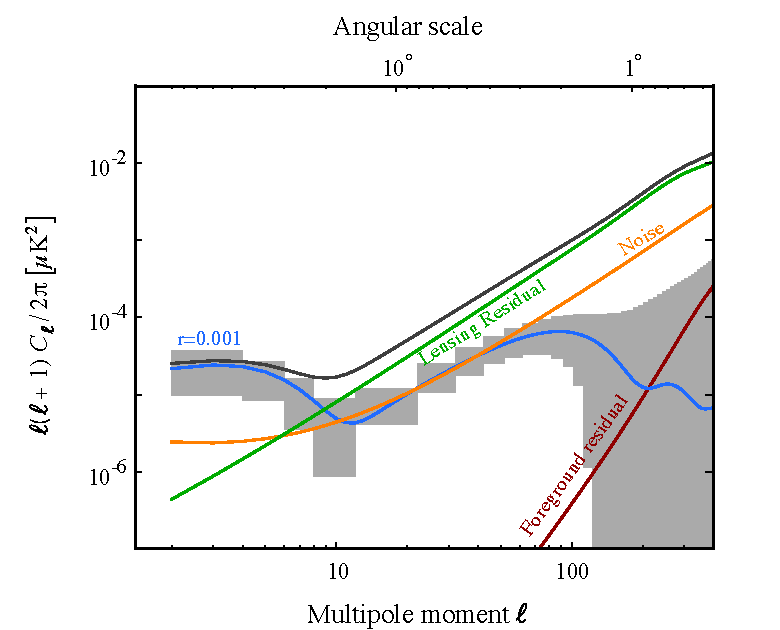
\includegraphics[width=3in]{figs/cmbbb_powspec_v1.pdf}
\end{center}
\vspace{-0.25in}
\caption{ \small \setlength{\baselineskip}{0.95\baselineskip}
Predicted determination of the \ac{CMB} power spectra for EPIC-IM (grey boxes) after foreground removal for $r=0$ (left) and after foreground removal and delensing for $r=0.001$ (right) overlaid on theoretical predictions (solid lines) and including Planck measurements of the temperature and $E$ modes (dark blue) and of several ground-based measurements of the lensing $B$ modes.  The primordial $B$ mode predictions (blue) are shown for two representative values of the tensor-to-scalar ratio: $r=0.001$ and $r=0.05.$ 
\label{fig:clall} }
\vspace{-0.05in}
\end{figure}

%\vspace{-0.1in}

In slow-roll inflation there are two classes of models that naturally explain the measured value of the spectral index $n_{\rm s}$. 
One is the set of potentials $V(\phi)\propto\phi^p$, which contains many of the canonical inflation models. This 
set is already under significant observational pressure. If the error bars on the spectral index tighten by a factor of about 2, 
and the 95\% C.L. upper limit on $r$ is pushed to even $\sim0.01$, all such models would be ruled out. The most recent constraint on the tensor-to-scalar ratio is $r < 0.07 \, (95\%)$; see Figure~\ref{fig:nsrp001}~\cite{Array:2015xqh}. \\

\begin{figure}[ht!]
\parbox{4.in}{\centerline {
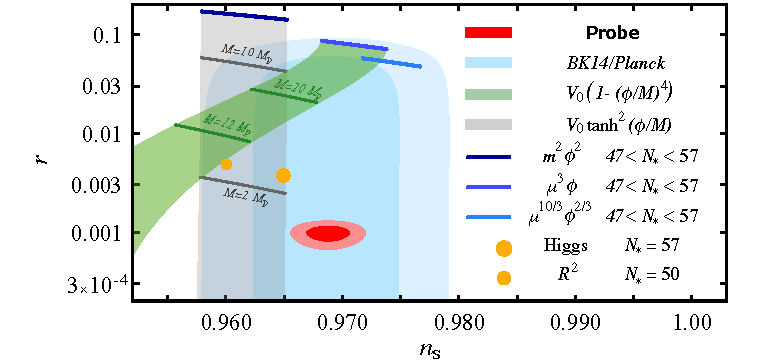
\includegraphics[width=4.2in]{figs/nsrlabeledrp001v2} } }
\hspace{-0.05in}
%\end{center}
\parbox{2.5in}{
\caption{ \small \setlength{\baselineskip}{0.95\baselineskip}
Current $1$ and $2\sigma $ limits on $r$ and $n_{\rm s}$ (blue)~\cite{Array:2015xqh} and forecasted constraints for a fiducial model with $r=0.001$ for 
EPIC-IM. Also shown are predictions for the models of the inflaton potential discussed in the text: Chaotic inflation (blue lines); 
Higgs and $R^2$ (large and small dots, respectively);  quartic hilltop (green band); and a sub-class of $\alpha$-attractor
models~\cite{Kallosh:2013hoa}
\label{fig:nsrp001} } }
%\vspace{-0.1in}
\end{figure}

Another class of models includes Starobinsky and Higgs inflation, which both have $r\sim0.003$. A future mission 
capable of reaching $\sigma_r\sim\mathcal{O}(10^{-4})$ would provide significant constraints on virtually all models that naturally explain $n_{\rm s}$. For a simple foreground model with spatially uniform spectral dependence assuming synchrotron emission that is well described by a power law and dust emission well characterized by a two-component model, EPIC-IM would achieve $\sigma(r)\sim1.3 \times 10^{-4}$ assuming $r=0.001$ and delensing with data from EPIC-IM itself. 
%Such a model is highly optimistic and including a simple model of spatially varying frequency dependence degrades the limits by $\sim 2$.  

%A detection of $B$ modes consistent with a primordial spectrum of vacuum fluctuations would be the first observation 
%of a phenomenon directly related to quantum gravity. 
A detection of $B$ modes consistent with a primordial spectrum of vacuum fluctuations would be the first observation of a phenomenon directly related to quantum gravity. In addition, a Probe mission would allow a high significance detection of any model of large-field inflation.
%In addition, any detection with a next generation satellite would be 
%evidence for {\it large-field} inflation~\cite{Lyth:1996im}, in which a smooth potential that supports inflation extends over 
%a distance in field space $\Delta\phi \gtrsim M_{\rm P}$. Studies of inflation in the context of quantum gravity give a generic 
%expectation $\Delta\phi \lesssim M_{\rm P}$~\cite{Banks:2003sx,Baumann:2014nda,Brown:2015iha,Rudelius:2015xta}, although 
%there are some mechanisms to realize large-field inflation \cite{Silverstein:2008sg,Kaloper:2008fb,Marchesano:2014mla,Blumenhagen:2015xpa}. 
A detection of $r$ would therefore provide 
motivation to better understand how large-field inflation can be naturally incorporated into quantum gravity~\cite{Banks:2003sx,Baumann:2014nda,Brown:2015iha,Rudelius:2015xta,Silverstein:2008sg,Kaloper:2008fb,Marchesano:2014mla,Blumenhagen:2015xpa}. 

Inflation predicts a $B$ mode spectrum with the shape shown in Figure \ref{fig:clall}, but there may be additional sources of $B$-mode polarization either during or after 
inflation. To be confident of the implications of a detection, the shape and Gaussianity of the $B$ mode spectrum 
must be characterized. The vast majority of inflation scenarios predict a Gaussian and nearly scale-invariant spectrum for 
gravitational waves. A target constraint of $\sigma(n_{\rm t})<1$ at $r=0.01$, easily achievable with a Probe mission, would significantly constrain non-vacuum 
inflationary sources~\cite{Namba:2015gja,Peloso:2016gqs}.
% and rule out physics completely inconsistent with inflation. 

Deeper mapping of $E$-mode polarization will also test inflationary models. Large scale $E$ modes will provide new tests of isotropy, a prediction of most models of inflation; 
for example, observations with a CMB Probe could reject at 99\% confidence models designed to explain the alignment of low multipoles in the temperature maps~\cite{Dvorkin:2007jp}. 
Together with continued improvements at high $\ell$ from the ground, these modes will also improve constraints on the scalar 
spectral index, its changes with scale, and on primordial non-Gaussianity by factors of about two. 

\begin{figure}[ht!]
\hspace{-0.2in}
\parbox{4.0in}{\centerline {
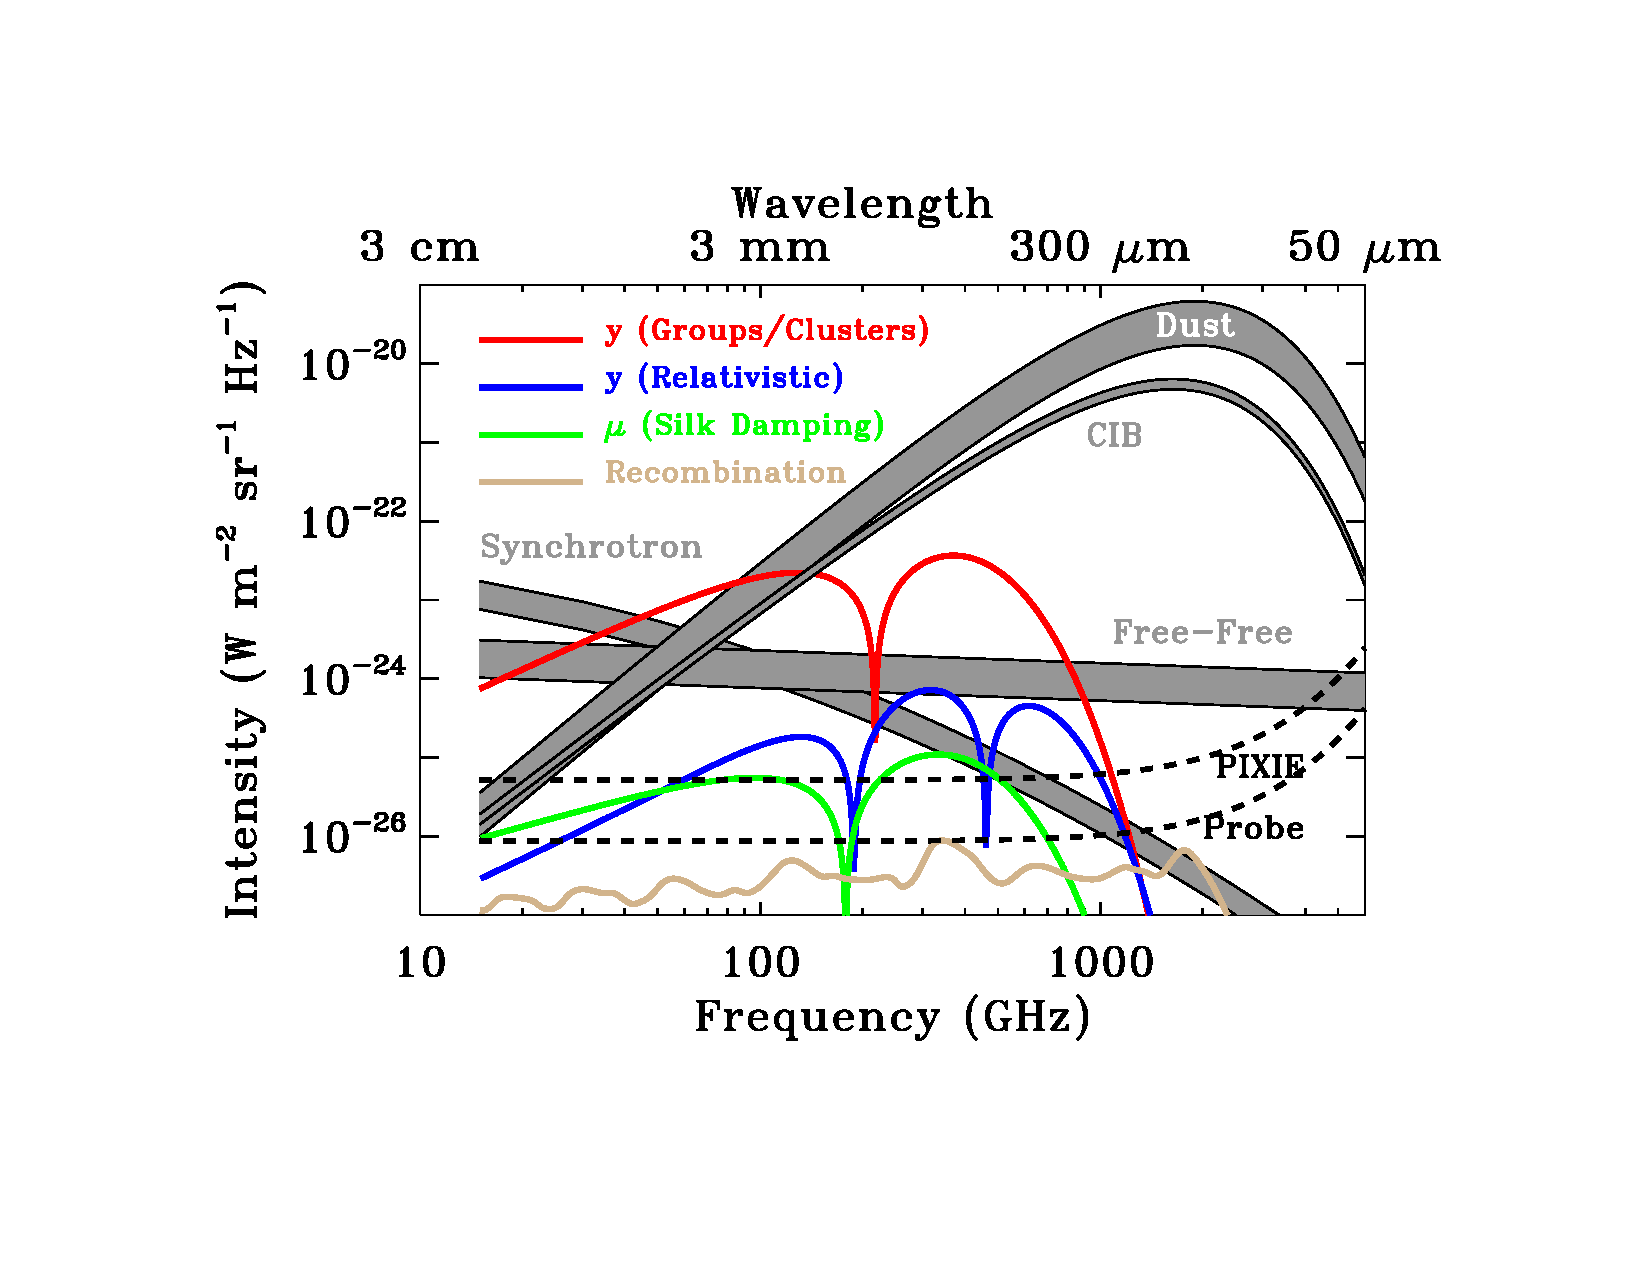
\includegraphics[width=3.0in]{Figures/probe_spectral_foregrounds_v3.pdf} } }
\hspace{-0.05in}
\parbox{2.5in}{
\caption{ \small \setlength{\baselineskip}{0.95\baselineskip}
Anticipated $y$ and $\mu$ spectral distortions (solid), the signature of resonant recombination lines (solid), and anticipated foreground 
signal levels relevant for spectral distortion measurements (grey bands). 
The simplest extension of a proposed
Explorer class mission (Probe, dash grey) gives approximately 10 times the Explorer sensitivity (PIXIE). 
A better optimized Probe may give detections of all anticipated distortions. 
\label{fig:distortions} } }
\vspace{-0.1in}
\end{figure}

Spectral distortion measurements give additional tests of inflation. The dissipation of small-scale 
perturbations through Silk-damping leads to $\mu$-distortions~\cite{Sunyaev1970diss, Daly1991, Hu1994, Chluba2012}. 
In $\Lambda$CDM the distortions are predicted at a level of $\mu=(2.0\pm0.14)\times 10^{-8}$, a level that 
is readily accessible to a Probe class mission, see Fig.~\ref{fig:distortions}~\cite{Chluba2012, Chluba2016LCDM}. 
A Probe may also give the sensitivity to detect the signature of recombination 
radiation imprinted by recombination of hydrogen and helium 
at redshift $z\simeq 10^3-10^4$; see Fig.~\ref{fig:distortions}~\citep{Sunyaev2009, Chluba2016}. 
The detailed physics is sensitive to the values of $n_{\rm s}$, which is a direct probe of inflation. 


%in the CMB spectrum, which provide a unique means to place stringent constraints on the amplitude of the small-scale curvature power spectrum. This information is on small scales (wavelength $0.1 \,{\rm kpc} \lesssim \lambda \lesssim 1\, {\rm Mpc}$) and from early times ($10^4 \lesssim z\lesssim 10^6$), inaccessible through any other observation. 

%In $\Lambda$CDM \citep{Chluba2012, Chluba2016LCDM}, distortions are predicted at a level of $\mu=(2.0\pm0.14)\times 10^{-8}$ (see Fig.~\ref{fig:distortions}). A detection would deliver a complementary test for the inflation paradigm~\citep{Chluba2012inflaton, Dent2012, Chluba2013PCA, Clesse2014, Cabass2016}, and new probes of the particle spectrum of inflation through new tests of non-Gaussianity~\citep{Pajer2012, Ganc2012, Biagetti2013, Razi2015, Chluba2016ng}. 
%It would also bring us to the sensitivity level required to detect the cosmological recombination radiation \citep{Sunyaev2009, Chluba2016} imprinted by the recombination of hydrogen and helium at redshift $z\simeq 10^3-10^4$, which can be used to probe the physics of recombination (see Fig.~\ref{fig:distortions}). 
%In summary, a detection of primordial gravitational waves consistent with the standard inflationary prediction would reveal the presence of a new fundamental energy scale for particle physics and would have far reaching implications for quantum gravity. Detecting correlations on the largest scales would confirm a primordial origin. Any departure from a nearly scale-invariant, nearly Gaussian spectrum would reveal new physics beyond the simplest inflationary model. In the absence of a detection, an improvement by about two orders of magnitude on the current upper limit would qualitatively change how we think about the inflationary paradigm.

\vspace{-0.15in}

\subsubsection{Light Relics and Dark Matter}

\vspace{-0.05in}

In the inflationary paradigm, the universe was reheated to temperatures of at least 10 MeV and perhaps as high as $10^{12}$ GeV.  
At these high temperatures, even very weakly interacting or very massive particles, such as those arising 
in extensions of the standard model of particle physics, can be produced in large abundances~\cite{1979ARNPS..29..313S,Bolz:2000fu}.  As the universe expands and cools, 
the particles fall out of equilibrium, leaving observable signatures in the \ac{CMB} power spectra. 
Through these effects the CMB is a sensitive probe of neutrino and of other particles' properties.  

One particularly compelling target is the effective number of light relic particle species $\Neff$, also called the effective 
number of neutrinos. The canonical value with three neutrino families is $\Neff = 3.046$. Additional light particles 
%in thermal equilibrium with the Standard model particles at any point in our history, it will 
contribute a change to $\Neff$ of $\Delta \Neff \geq 0.027\,g$ where $g \geq 1$ is the number of 
degrees of freedom of the new particle~\cite{Brust:2013xpv,Baumann:2016wac}.  
This defines a target of $\sigma(\Neff) < 0.027$ for future CMB observations. 
Either a limit or detection of $\Delta \Neff$ at this level would provide powerful insights into the basic constituents 
of matter. 

Forecasts for $\Neff$ are shown in Figure~\ref{fig:Neff_future}.  The two most important parameters for improving constraints
are the fraction of sky observed $f_{\rm sky}$ and the noise. Achieving both larger $f_{\rm sky}$ and
lower noise are strengths of the CMB Probe compared to other platforms. 
Our baseline mission nearly reaches the target constraint with $g=1$, and
a newly designed mission is could reach $\sigma(\Neff) < 0.027$.  A high precision measurement of the CMB in temperature and polarization is the only proven approach capable of reaching this important threshold.  

\begin{figure}[t!]
\begin{center}
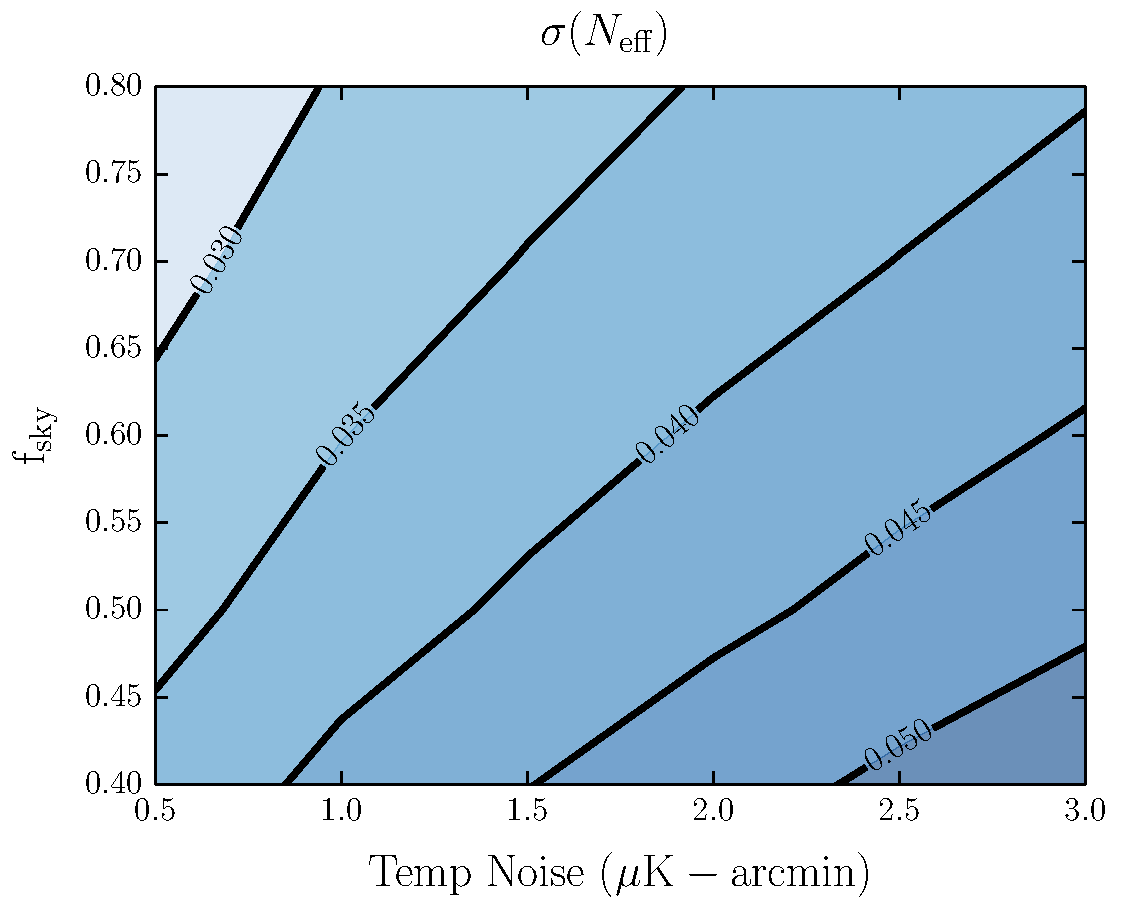
\includegraphics[width=0.45\textwidth]{figs/Neff.pdf}
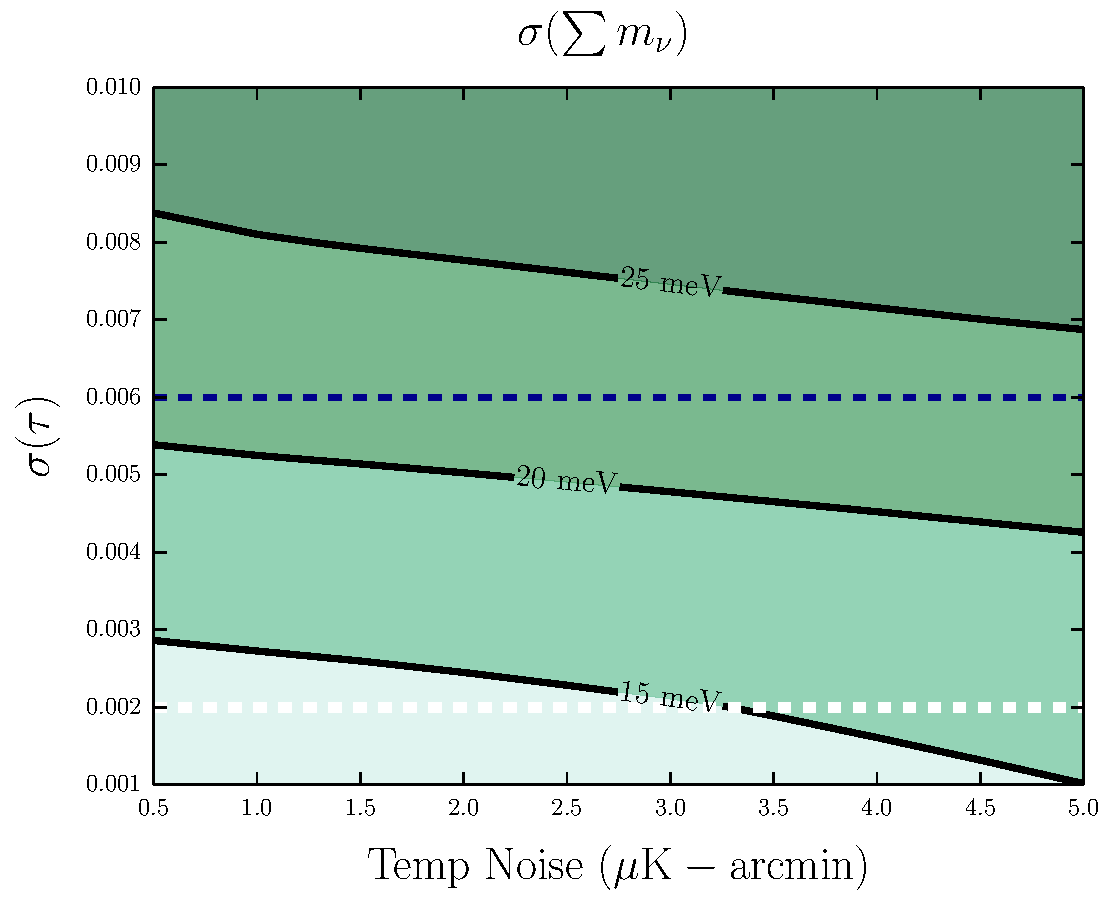
\includegraphics[width=0.45\textwidth]{figs/Mnu_tauprior.pdf}
\caption{ \small \setlength{\baselineskip}{0.95\baselineskip}
$\Neff$ as a function of noise and sky fraction (left) and
Neutrino mass constraints as a function of uncertainties in measurement of $\tau$, noise, and 
sky fraction of $f_{\rm sky} = 0.7$. The resolution assumed is 5'.  
Vertical lines denote the expected performance of EPIC-IM. 
The blue dashed line is the current \planck~limit; the grey dashed line is the limit from cosmic variance 
measurement of $\tau$. All forecasts assume internal delensing of the $T$ and $E$-maps~\cite{Green:2016cjr}, 
including residual non-Gaussian covariances.  The $\sum m_\nu$ forecasts include DESI BAO.  
\label{fig:Neff_future} }
\end{center}
\vspace{-0.15in}
\end{figure}

Many light relics of the early universe are not stable. They decay, 
leaving faint evidence of their past existence on other tracers. The relics with sufficiently long lifetime to survive few minutes, 
past the epoch of light element synthesis, leave a signature on the helium fraction $Y_p$.  If they decay 
by the time of recombination, their existence through this period is best measured through the ratio of $\Neff$ to $Y_p$. 
The Probe's cosmic variance limited determination 
of the $E$ mode power spectra will improve current limits for these quantities by
a factor of five thus eliminating sub-MeV mass thermal relics. 
%  
Spectrum distortion measurements give additional constraints on the lifetime and abundance 
of such relics \citep{Sarkar1984, Kawasaki1986, Hu1993b, Chluba2011therm}. A future Probe's $\mu$-distortion constraint gives a two orders of magnitude improvement on the abundance and lifetime of early universe relics \cite{Chluba2013fore, Chluba2013PCA} compared to current constraints derived from measurements of light element abundances \cite{Kawasaki2005, Jedamzik2006}.

Cosmological measurements have already confirmed the existence of one relic that lies beyond the 
Standard Model: dark matter. For a conventional WIMP candidate, the CMB places very stringent 
constraints on its properties through the signature of its annihilation on the $T$ and $E$ 
spectra \citep{Peebles2000, Chen2004, Padmanabhan2005}.  Planck currently excludes WIMPs with mass 
$m_{\rm dm}< 16$ GeV and a future CMB mission could reach $m_{\rm dm} < 45$ GeV for $f_{\rm sky} =0.8$.  The 
CMB provides the most stringent constraints on the dark matter annihilation cross section for dark matter 
in this mass range.  The CMB is complimentary to direct detection experiments which probe the scattering 
cross-section of dark matter with standard model particles.

%A dark matter candidate can also have a slow decay to Standard models particles which is 
%similarly constrained by the CMB~\cite{Chen2004, Zhang2007, Diamanti2014, Slatyer:2016qyl}.  Current and future CMB limits on the lifetime of $\tau \gtrsim 10^{25}$ s are somewhat weaker than indirect detection limits of $\tau > 10^{24-28}$~s~\cite{Essig:2013goa}.  

A particle-independent approach is to constrain dark matter interactions that would 
affect the evolution of the effective dark matter fluid and its interactions with baryons or photons.  The simplest example is 
to constrain the baryon-dark matter cross section through its effective coupling of the two fluids~\cite{Dvorkin:2013cea}.  
These couplings affect the evolution of fluctuations and ultimately the $T$ and $E$ spectra. The current limits of $\sigma \lesssim 10^{-31}-10^{-34}\,{\rm cm}^2 \times (m_{\rm dm} / {\rm MeV})$ can be competitive with direct detection for sub-GeV masses.  
More exotic dark sectors that include long-range forces can produce an even richer phenomenology in the CMB and in the large-scale structure 
without necessarily producing an associated signature in direct detection experiments or 
indirect searches (e.g.~\cite{Cyr-Racine:2013fsa,Buen-Abad:2015ova,Lesgourgues:2015wza}). 

Interactions of dark matter with standard model particles can also be constrained through 
measurements of spectral distortions \cite{Yacine2015DM}. 
%Chluba et al. showed 
%As the universe expands, the matter cools. Compton interactions with electrons keep the normal matter at the CMB 
%temperature until well after recombination. This leads to a small distortion of the CMB with a negative chemical 
%potential~\citep{Chluba2011therm}. In a similar manner, interactions of DM with electron, protons or directly 
%with CMB photons can lead to a distortion. 
Current constraints from FIRAS are most sensitive to small dark matter
mass, $m_{\rm X}\lesssim 0.2\,{\rm MeV}$, but these could be extended to $m_{\rm X}\lesssim 1\,{\rm GeV}$ with a 
Probe-class mission, testing DM interaction down to cross-sections 
$\sigma\simeq 10^{-39}-10^{-35}\,{\rm cm}^2$~\cite{Yacine2015DM}. This provides new constraints on the low mass end, $m_{\rm X}\lesssim 10\,{\rm MeV}$ and improve existing limits~\cite{Essig2012PhRvL.109b1301E, Boehm2014MNRAS.445L..31B} by up to a factor of $\simeq 50$. Distortion measurements furthermore open a new avenue for testing dark matter-proton interactions~\cite{Yacine2015DM}.

A host of other physical phenomena including the existence and properties of axions, primordial magnetic fields, and 
superconducting strings, leave signatures on the spectrum of the CMB and can therefore be constrained by 
the sensitive measurements  of a future Probe~\cite[e.g.,][]{Jedamzik2000, Tashiro2012, Dolgov2013, Tashiro2013, Caldwell2013}.


\vspace{-0.15in}

\subsubsection{Neutrino Mass}

\vspace{-0.05in}

%One of the last unknowns of the Standard model of particle physics is the absolute mass scale of the neutrinos.  
%While measurements of neutrino oscillations demonstrate the neutrinos have mass, directly measuring the scale of the masses is challenging experimentally.  
%Current measurement of $\Neff$ confirm the existence of a cosmological abundance of neutrinos whose gravitational influence is detectable in the CMB and in large scale structure.  
Cosmology is uniquely capable of measuring the sum of neutrino masses, $\sum m_\nu$, directly through the 
suppression of the growth of structures in the universe on small scales.   However, all cosmological measurements of $\sum m_\nu$ are fundamentally limited by our uncertainty in $\tau$ due to the strong degeneracy between $\tau$ and $A_s$.  Although many surveys hope to detect $\sum m_\nu$ at high significance, any detection of the minimum value expected from particle physics  
$\sum m_\nu = 58$~meV at more than $2 \sigma$ will require a better measurement of $\tau$.  The best constraints on $\tau$ come from $E$ modes with $\ell < 20$ which require 
measurements over the largest angular scales.
To date, the only proven method for such a measurement is from space, including the current limit  from \planck\ of $\sigma({\tau}) = 0.009$~\cite{planck2016_xlvi}.  Forecasts for an internal 
CMB measurement of $\sum m_\nu$ via CMB lensing~\cite{Kaplinghat:2003bh} are shown Figure~\ref{fig:Neff_future}.  With the current measurement of $\tau$ one is limited to  
$\sigma(\sum m_\nu) \gtrsim 25$ meV, with similar conclusions holding for other types of cosmological measurements.  The \ac{CMB} Probe will reach the cosmic variance limit of $\tau \sim 0.002$ and will therefore 
reach $\sigma(\sum m_\nu) < 15$ meV when combined with DESI's measurements of 
baryon acoustic oscillations~\cite{Levi:2013gra}.  Robustly detecting neutrino mass at  $> 3\sigma$ in any cosmological setting is only possible with an improved measure of $\tau$ like one one achievable with the \ac{CMB} Probe.

%A detection of $\sum m_\nu$ at this level is not possible with any other existing survey.

%Larger $\sum m_\nu$ gives a larger suppression and the $\sum m_\nu$ can be measured by 
%The \ac{CMB} Probe would be a valuable tool in the quest for a cosmological detection of $\sum m_\nu$.   
%The sensitivity to $\sum m_\nu$ from suppression of power is limited by our knowledge of 
%the primordial amplitude of fluctuations $A_s$, which is strongly degenerate with the optical depth $\tau$.  
%The current limit on $\tau$ from \planck\ of $\sigma({\tau}) = 0.009$~\cite{planck2016_xlvi} limits 
%$\sigma(\sum m_\nu) \gtrsim 25$ meV. Forecasts for an internal 
%CMB measurement of $\sum m_\nu$ via CMB lensing~\cite{Kaplinghat:2003bh} are shown Figure~\ref{fig:Neff_future} but the conclusion is the same for any proposed cosmological probe.
%This lower limit is common to any measurement that depends on the relative suppression.  
%Therefore, a cosmological detection of the minimum value expected from particle physics  
%$\sum m_\nu = 58$~meV at more than $2 \sigma$ will require a better measurement of $\tau$.  

%The \ac{CMB} Probe will reach the cosmic variance limit of $\tau \sim 0.002$ and will therefore 
%reach $\sigma(\sum m_\nu) < 15$ meV when combined with DESI's measurements of 
%baryon acoustic oscillations~\cite{Levi:2013gra}.  
%A detection of $\sum m_\nu$ at this level is not possible with any other existing survey.
%if not accompanied by an improvement to the measurement of $\tau$.

\vspace{-0.15in}

\subsubsection{Cosmological structure formation}

\vspace{-0.05in}

Understanding the evolution of cosmological structures from small density perturbations through the formation of the
first stars to present day galaxies and clusters is a key goal of cosmology~\cite{dunlop2011}. 
Cosmological reionization, the transition of the universe from dominated by neutral to ionized 
hydrogen, is a cornerstone of this evolution because it encodes information 
about star formation history and the physical processes that formed galaxies of various luminosities and masses. 
But when did the epoch of reionization start?  How long did it last? Are early galaxies enough to reionize the entire universe
or is another source required?
 
Measurements of the \ac{CMB} $E$ mode power spectrum over large angular scales are sensitive to the optical depth 
to reionization $\tau$, a key parameter for all reionization models that attempt to answer these questions. 
The \planck\ team  reported recently a value of $\tau=0.055 \pm 0.009$~\cite{planck2016_xlvi,planck2016_xxxi}.
The level is lower than previous estimates and reduces the tension between CMB-based analyses and constraints from 
other astrophysical sources.  
%While the average redshift at which reionization occurs is found to be $z_re\simeq 8$ assuming an 
%instantaneous reionization, suggesting that reionization occurred rather late.
The CMB Probe's cosmic variance limited measurement of $E$-mode polarization will 
improve the $1\sigma$ error by a factor of 4.5 to reach a cosmic 
variance limited measurement of $\tau$, thus setting 
stringent constraints on models of the reionization epoch. 
% that require additional sources of reionization, non-standard early galaxies, 
%or significantly evolving escape fractions or clumping factors. On the whole a better estimate of $\tau$ when combined with direct probes at low redshift, 
%will help to characterize the duration of the epoch of reionization and tell us when it started.

%will  set stringent constraints on models of the reionization epoch. \comred{what is the quantitative connection to models of reionization}.

%The optical depth to reionization, $\tau$, places an important integral constraint on the extended reionization history.
%The {\it Planck} Collaboration~\cite{planck2015-XLVI,planck2015-XXXI} reported recently a value of $\tau=0.055 \pm 0.009$ significantly lower than previous estimates. 
%This suggests that an early onset of reionization is strongly disfavoured by the {\it Planck} data. 
%The {\it Planck} Collaboration~\cite{planck2015-XXXI} showed that this result reduces the tension between CMB-based analyses and constraints from 
%other astrophysical sources. 
%A cosmic variance limited measurement of $E$-mode polarization on large scales, possible with a probe mission, will render the most accurate 
%determination of $\tau$ (Figure~\ref{fig:Neff_future}
%shows a cosmic variance limit measurement of $\tau$ along with the current {\it Planck} limit, break the degeneracy with the neutrino mass, 
%set stringent constraints on models of the reionization epoch, and, finally, help understanding the formation of the cosmological structures we see today.

The anisotropy in the \ac{CIB} produced by dusty star-forming galaxies in a wide redshift range, are
an excellent probe of both the history of star formation and the link between
galaxies and dark matter across cosmic time. The \planck\ collaboration 
derived values of the star formation rate that,
at redshifts z$\mathrm{\sim3}$, are three times larger 
than constraints from number counts measurements (\cite{planck2014-XXX,planckXVIII,madau2014}).
By measuring \ac{CIB} anisotropy with 100 times higher signal-to-noise ratio
the CMB Probe will shed light on this intriguing discrepancy. 
Specifically, it will constrain the star formation rate with one tenth of \planck 's uncertainty. 


A key parameter in simulations of the angular power spectrum of the \ac{CIB} 
is $M_{\mathrm{eff}}$, the galaxy halo mass that is most efficient in producing star 
formation activity. Comparing measurements of the power spectrum to simulations
constrains this parameter, which informs structure formation models. Current models and measurements 
find $M_{\mathrm{eff}}\sim 10^{12}$ solar masses with about $\mathrm{10\%}$ uncertainty. 
The CMB Probe will constrain this parameter at the percent level.


%Dusty star-forming galaxies trace the underlying dark matter
%field in a broad redshift range. Therefore, a wealth of information will be extracted by 
%correlating the anisotropy in the \ac{CIB} 
%with multiple dark matter tracers including catalogs of galaxies and quasars, 
%and maps of the $\gamma$-ray and the X-ray background~\cite{serra2014,wang2015,cooray2016}.
%These cross-correlations will provide an additional probe of the star formation history, and they will shed light on the interaction between 
%light and matter in a broad wavelength range. \comred{the paragraph starts with dark matter, but ends 
%with SFR ..?}

Reionization of the universe and the onset of structure formation inject
energy into the sea of CMB photons. This injection is detectable through a distinct spectral distortion. 
This is the largest expected distortion -- marked `$y$ Groups/Clusters' in Figure~\ref{fig:distortions} --
and will be clearly detected by the CMB Probe. 
A detection will give information about the total energy output of the first stars, AGNs, and galaxy clusters, 
an important parameter in structure formation models. 

Group-size clusters that have masses $M\simeq 10^{13}\,M_{\odot}$ contribute significantly to the signal. 
With temperature $k T_{\rm e}\simeq 1\,{\rm keV}$ these are sufficiently hot to create a relativistic 
temperature correction to the large $y$-distortion. This relativistic correction, denoted `$y$ relativistic' in 
Figure~\ref{fig:distortions},  will also be detected with high signal-to-noise ratio by the CMB Probe, and 
will be used to constrain the currently uncertain feedback mechanisms used in hydrodynamical simulations
of cosmic structure formation~\citep{Hill2015}. 

%Large-scale structure can also be probed using CMB spectral distortions measurements. 
%In fact, the largest guaranteed distortion is caused by the associated late-time energy release of 
%forming structures and from reionization~\cite{Sunyaev1972b, Hu1994pert, Oh2003, Cen1999, Refregier2000}, 
%imprinting a $y$-type distortion with $y \simeq 2\times 10^{-6}$ \citep[e.g.,][]{Refregier2000, Hill2015}. 
%This distortion is only one order of magnitude below the current limit from COBE/FIRAS and, even with most 
%pessimistic assumptions about foregrounds, should be clearly detected with the next-generation spectrometers we propose to study. 
%A detection will give information about the total energy output of first stars, AGN and galaxy clusters. \comred{what do 
%you do with this number? how does this feedback to constraints on SFR or other parameters of structure evolution models?}
%In particular, group-size clusters that have masses $M\simeq 10^{13}\,M_{\odot}$ contribute significantly to the signal. 
%With temperature $k T_{\rm e}\simeq 1\,{\rm keV}$ these are sufficiently hot to create a relativistic 
%temperature correction to the large $y$-distortion. This relativistic correction, denoted `$y$ relativistic' in 
%Figure~\ref{fig:distortions},  
%which can be used to constrain the currently uncertain feedback mechanisms used in hydrodynamical simulations
%of cosmic structure formation~\citep{Hill2015}.  (see Fig.~\ref{fig:distortions}).

The CMB spectrum varies spatially across the sky. One source of such anisotropic distortion is due to 
the spatial distribution clusters of galaxies and has already been measured by Planck~\cite{Planck2013SZ}. 
A combination of precise CMB imaging 
and spectroscopic measurements will allow observing the relativistic temperature correction of individual SZ 
clusters~\cite{Sazonov1998,Itoh98,Challinor98}, which will calibrate cluster scaling relations and inform our 
knowledge of the dynamical state of the cluster atmosphere. 

Resonant scattering of the CMB photons during and post last scattering leads to spectral-spatial signals
that can be used to constrain the abundance of metals in the dark ages and therefore the make-up of the 
first, and subsequent generations of stars~\cite{Jose2005, Carlos2007Pol, Lewis2013,Kaustuv2004, Schleicher2008}. 


\vspace{-0.22in}

\subsection{The Challenges: Foregrounds and Systematics}
\label{sec:foregrounds}
\vspace{-0.05in}

%A satellite mission provides a unique opportunity to target both the inflationary B-mode polarization that originates from the epoch of recombination and peaks around $\ell=80$ and the contribution that peaks on significantly larger scales $\ell\lesssim 12$. To measure the contribution from reionization will require an unprecedented understanding of foregrounds and systematic effects. This is illustrated in the left panel of Figure~\ref{fig:Qrp001}, which shows the contribution from reionization to the Stokes $Q$-parameter for $r=0.001$. The amplitude of the signal is approximately $10$ nK

The search for primordial $B$-modes is one of the main science
objectives of future CMB missions. A satellite experiment enables
full-sky observations, and provides complete flexibility in the choice
of frequency coverage, both of which are challenging from the ground
or from the balloon platform.  Among other limitations, the atmosphere
prevents observations at key frequencies, such as 60\,GHz, and
requires data filtering that makes it difficult to recover the larger
angular scales.

By the time a probe-class mission launches, substantial progress will
have been made in this quest.  In the absence of a primordial $B$-mode
signal at detectable levels, the mission will significantly improve
the upper limit on the tensor-to-scalar ratio $r$, with
$\sigma(r)\!\sim\!10^{-3}$.  However, if $r$ is large enough,
tentative $B$-mode detections could be reported from the ground or by
ballon experiments ahead of this mission. The significance of such a
discovery would be such that the detailed characterization of the
angular and spectral dependence of the signal, as well as the
verification of its isotropy across the sky, both of which are
uniquely enabled by a satellite mission, would be required to confirm
its primordial origin \comred{(cite Decadal Survey)}.

In this scenario, a probe-class mission will in particular detect and
characterize the reionization signal expected at the largest angular
scales (multipoles below $\sim\!10$), where observations from other
platforms are the most challenging. The contribution from reionization
to the Stokes parameter $Q$ for $r=0.001$ is shown in the left panel
of Figure~\ref{fig:Qrp001}. The amplitude of this signal is
$\sim\!10$\,nK, which requires that any experiment attempting to
measure it control large-scale foregrounds and systematics at the
unprecedented level of a few nK.

\begin{figure}[h]
\begin{center}
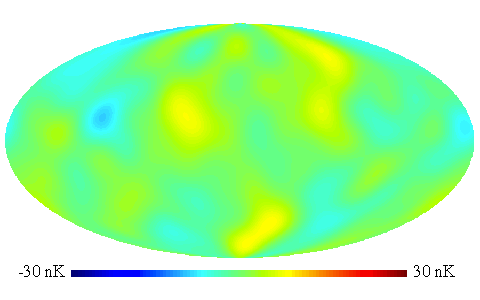
\includegraphics[width=3.2in]{Figures/P15_2_12_rp001.pdf}
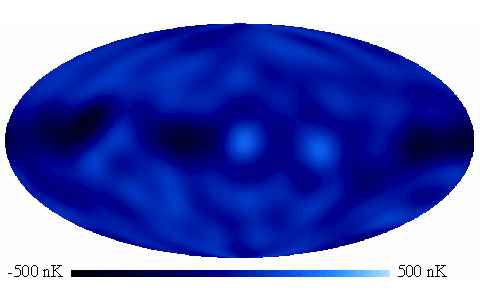
\includegraphics[width=3.2in]{Figures/P353_N_2_12.pdf}
\end{center}
\caption{{\it Left panel:} Contribution to the Stokes $Q$ parameter
  from inflationary $B$-modes for $\ell<12$ and $r=0.001$. {\it Right
    panel:} Noise in the $Planck$ 353 GHz map of the Stokes $Q$
  parameter for $\ell<12$ rescaled to 150\,GHz assuming the spectral
  properties of dust.}
\label{fig:Qrp001}
\end{figure}

\subsubsection{Foregrounds}

Data from the \emph{Planck} satellite have significantly improved our
understanding of foregrounds in both intensity and polarization.
 %In intensity, $Planck$, for example, showed the unexpected relevance of Carbon-Monoxide lines at moderate latitudes as well as the existence of an anomalous emission from dust at low frequencies.
In polarization, the sky is dominated by the expected sources, namely
synchrotron and dust emission. \emph{Planck} has provided us with much
improved measurements of their amplitude and spectral dependence. The
observed frequency spectra of both foregrounds are shown for three sky
fractions in the left panel of Figure~\ref{fig:frequency}.  \emph{Even
  in the cleanest patches of the sky}, polarized foreground emission
is brighter than the sought-after primordial $B$-mode signal by over
an order of magnitude at all frequencies.  This statement holds at all
angular scales relevant to the search for primordial $B$-modes, as
shown in the right panel of Figure~\ref{fig:frequency}.

Perfect knowledge of the foreground components would enable their
removal from microwave data, but the sensitivity of the \emph{Planck}
measurements limits it at a level insufficient to detect primordial
$B$-modes, even for values of $r\!\sim\!10^{-1}$. The right panel of
Figure~\ref{fig:Qrp001} shows the noise in the \emph{Planck} 353\,GHz
map of the Stokes $Q$ parameter at the angular scales relevant for
primordial $B$-mode measurements, and rescaled to 150\,GHz assuming
the spectral dependence of dust; it is over an order of magnitude
larger than the inflationary contribution for $r=0.001$.  A mission
aiming to detect primordial $B$-modes at this level across the sky
will therefore not be able to rely on existing data. High
signal-to-noise foreground measurements must accompany those at
frequencies where the CMB contribution is larger.  As discussed below,
optimizing the frequency coverage of these measurements will be a key
goal of the mission concept study.

While the search for primordial B-modes leads to the strictest constraints on foreground residuals, exquisit control of foregrounds is also necessary for other science objectives. A satellite mission is likely also the only reliable way to measure the optical depth at a level necessary to break the degeneracy with the neutrino mass. Furthermore, a cosmic variance limited measurement of E-mode polarization on large scales possible with a probe mission would contain valuable information about the star formation history. 

Similarly, a clear objective of the spectral science is to have a robust, foreground-marginalized expectation of detecting the $\mu$-distortion generated by the dissipation of small-scale acoustic modes in $\Lambda$CDM. While an instrument like PIXIE just falls short of this objective, it seems within reach of a probe mission.

\begin{figure}[h]
\begin{center}
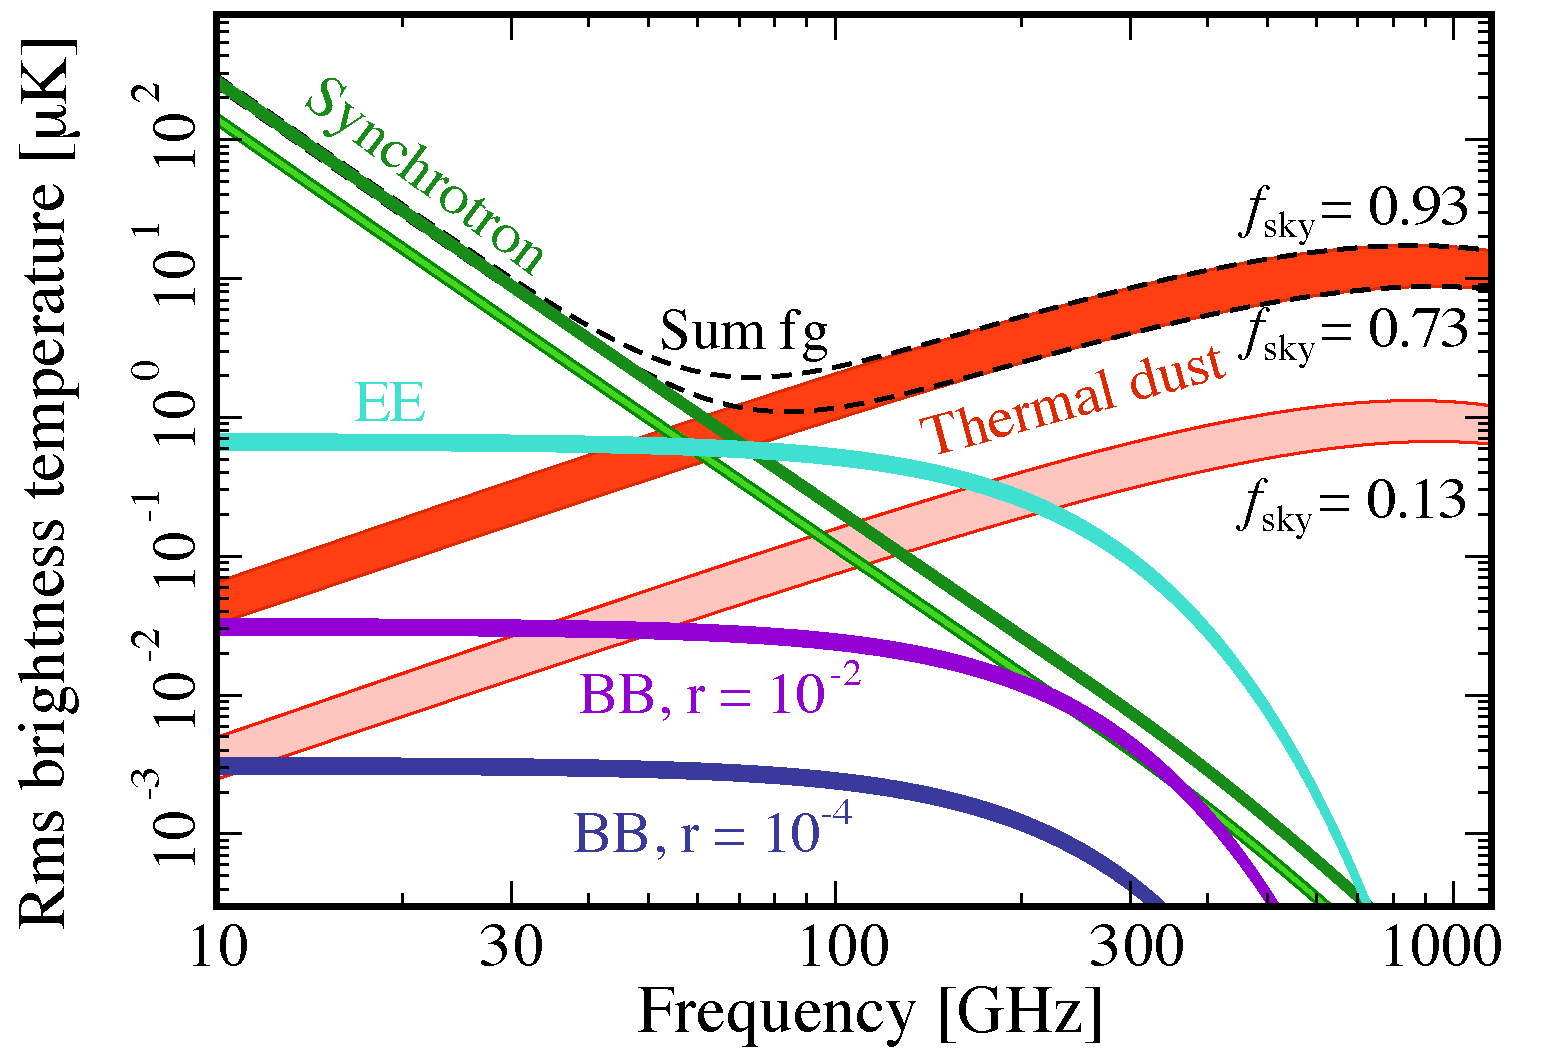
\includegraphics[width=3.26in]{Figures/overview_pol_v4_fsky_noplanck.pdf}\hskip .2cm
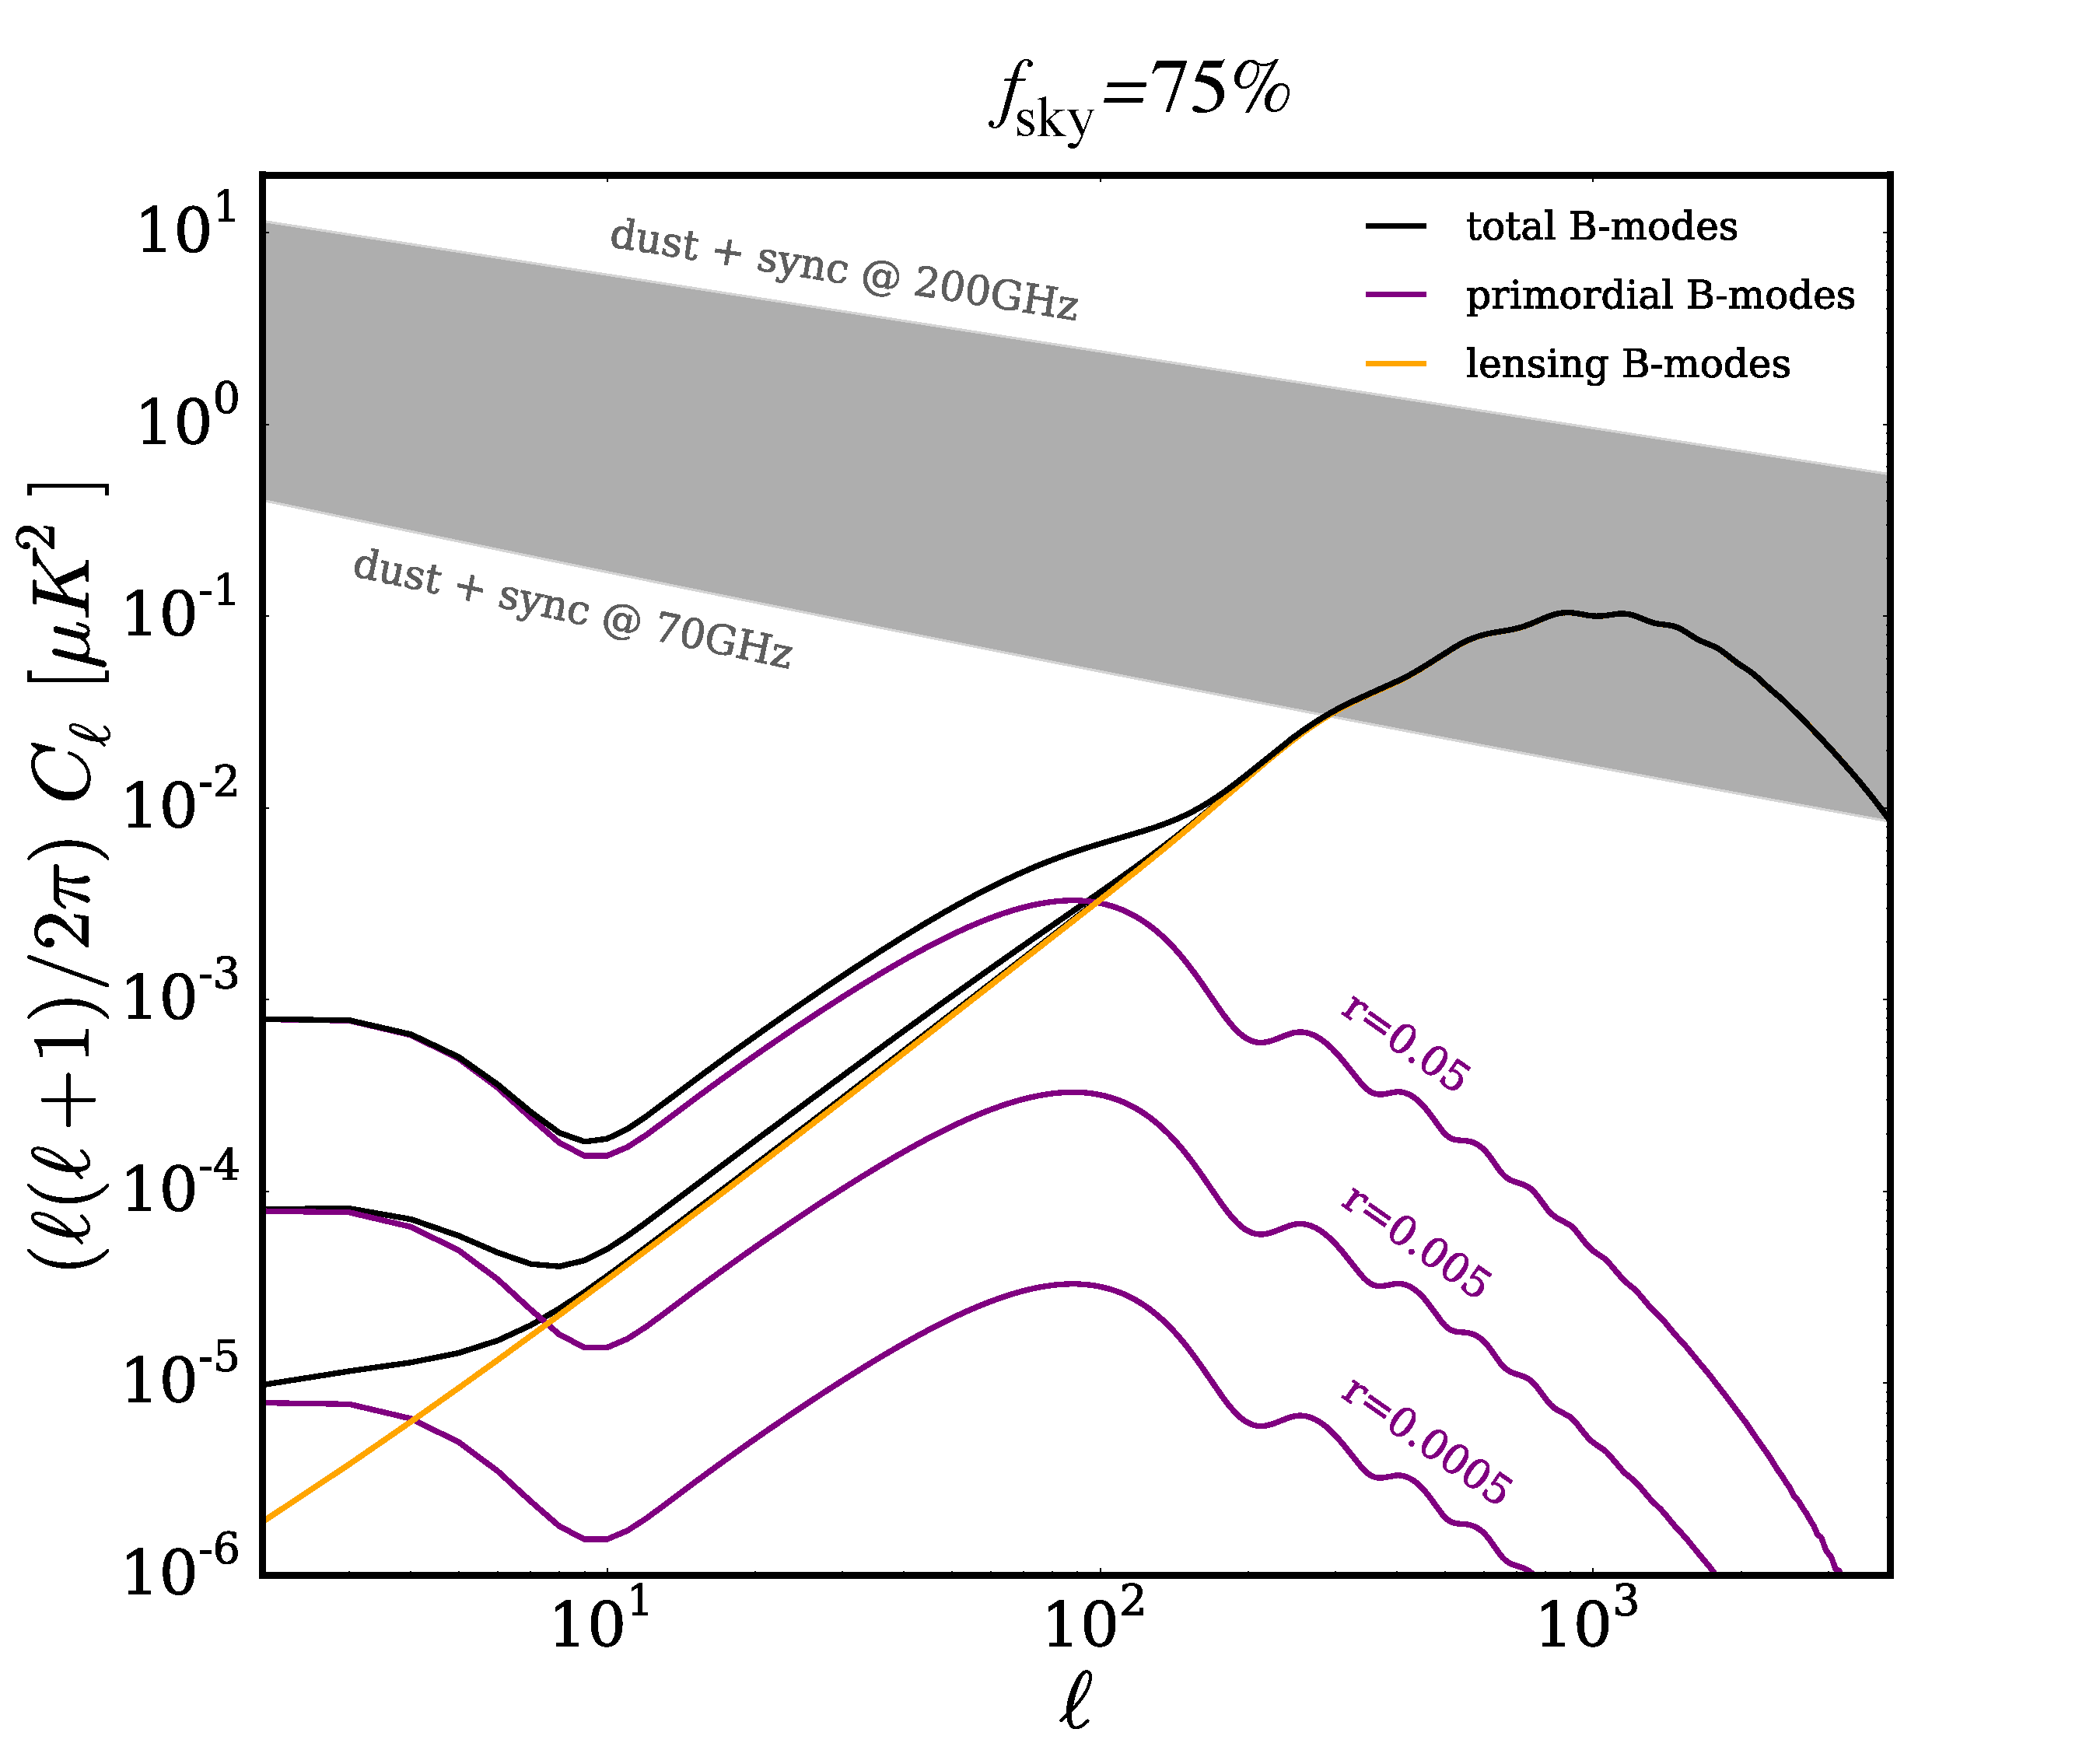
\includegraphics[width=3.12in]{Figures/clbb_freq.pdf}
\end{center}
\caption{{\it Left panel:} Brightness temperature as function of frequency for the CMB as well as synchrotron emission (green) and dust emission (red). The darker bands show the brightness temperature for sky fractions between $73\%$ and $93\%$, the lighter bands show the brightness temperature for the cleanest $13\%$ with the width indicating the uncertainty. {\it Right panel:} Angular power spectrum for B-mode polarization of the CMB for $r=0.0005$, $r=0.005$, and $r=0.05$ as well as for foreground emission between 70 and 200 GHz.}
%, which shows the power spectrum of
%foregrounds over $75\%$ of the sky for frequencies between $70$ and
%$200$ GHz together with the lensing and inflationary contribution for
%different values of the tensor-to-scalar ratio.
\label{fig:frequency}
\end{figure}


One of the key ingredients in the design of a CMB experiment is the frequency coverage required to achieve the science goals. Consequently, optimizing frequency coverage in light of the new information from $Planck$ and its limitations will be one of key task of the study proposed here.   

To achieve these goals we plan to investigate the effect on the measurements of r and $\tau$ of the presence of foregrounds residuals in the CMB maps (after foreground separation and/or cleaning) including, for example, the properties of the polarized thermal dust emission, specifically the potential spatial variation of its spectral index, hinted at by the observed decorrelation of the dust between 217 GHz and 353GHz Planck channels (\ref{Planck2015-X;Planck2015-L;Planck2015-XXIX;Boulanger2016}), and the study of the breakdown of the modified black body spectrum model. 
These aspects are better explored with the help of physically motivated models of the foregrounds (\ref{Bruce+Fraisse2009,Hensley et al in preparation}) and simulations based on these, using either existing simulation tools and/or implementing new simulators when required. 

The optimization of frequency channels will be conducted using both traditional (Fisher codes both spectra and map based) and novel techniques currently in development (such as direct Bayesian MCMC inference of cosmological parameters in the presence of foregrounds, (extension of the method presented in  \ref{Jewell2016}). Realistic simulations (including time domain based) are essential to fully assess the performance of a given instrument design/concept in view of both foreground residuals and the presence of systematics. We plan to generate these simulations, process them as we would do the real data, specifically applying some of the current component separation methods to clean the frequency maps from foreground emission (akin to {\it Planck} collaboration procedures \ref{Planck2015-IX}) and propagate to parameter estimation, assessing the impact of all contaminating effects on the accuracy and potential biases of the parameters estimated with particular emphasis on r and $\tau$.



%references
%Bruce+Fraisse2009 - 2009ApJ...696....1D
%Planck2015-IX - 2016A&A...594A...9P
%Planck2015-X - 2016A&A...594A..10P
%Planck2015-XXIX - A&A 586, A132 (2016)
%Planck2015-L - arXiv:1606.07335v1;
%Boulanger2016 - A&A 580, A136 (2015)
%Jewell2016 -  ApJ., 820, 2016
%





% Raphael, Josquin, Aurelien, Charles, Graca


\vspace{-0.22in}


\subsubsection{Systematic Errors}
% Brendan
\vspace{-0.05in}

The latest experience with \planck\ points to the following systematic error categories likely to be important for 
the CMB Probe, or for that matter, for any instrument striving to map the polarization 
over large portions of the sky to the levels targeted by the CMB Probe~\cite{PlanckintermediateXLVI}:
% only future space mission or anything targeting this $\sigma (r)$? 
1. Intensity-to-polarization leakage, 2. stability, and 3. straylight. 
Each of these is considered in light of polarimetry measurements through
differencing the signals of two detectors that are sensitive to orthogonal polarization states. 
% at different times and orientations are combined to recover
% the maximum likelihood polarization signal from each point on the sky.

\textbf{Leakage} \hspace{0.1in} The CMB anisotropy signal is a factor of 1000 larger 
than the strongest possible inflationary B-mode signal (see for example Fig.~\ref{fig:clall}). 
Therefore instrumental effects that can leak
even a small fraction of an intensity fluctuation into spurious  polarization
must be understood and controlled. The main effects are differences between gains of detectors, 
their frequency bandpass mismatch, their differential pointing on the sky, 
and their differential antenna patterns. These differential effects need to be controlled, through 
instrument design, characterization, and data analysis to 1 part in $10^{4}$ to give a negligible contribution for 
$\sigma(r) <0.001$.  This level of control represents a factor of 100 improvement on \planck 's performance~\cite{PlanckintermediateXLVI}. \comred{what about Bicep/Keck?}

Leakage-related effects will drive: requirements on the optical system, and the uniformity of the
bandpass of each polarimeter;  calibration requirements on the level of cross-polar leakage and its angle; 
% why are we saying 'cross-polar' leakage?
and measurements of the the beam shape as a function of source spectrum. 
These systematic effects can potentially be mitigated by modulation of the sky signal in
such a way that allows complete reconstruction of the 
polarized sky signal using each photometer, for example, using a
half-wave plate.  
% does all of this belong here or in 'to do'.

\textbf{Stability.}  %Given the need to avoid light from the Sun, Earth, and Moon, 
\comred{need more number(s) in this paragraph}
The reconstruction of deep, full sky polarization maps involves a combination of measurements made at times
separated by months, requiring stability of the response of the instrument on corresponding time scales.  Random deviations
from stability are a source of noise; systematic deviations are a source of systematic error. 
This type of systematic error puts requirements on control of thermal drifts of spacecraft temperatures, to
mitigate thermal emissivity changes and thermoelastic deformation of telescope structures.  
The cryogenic operating temperatures of detectors or reference calibration loads must be controlled
adequately as well. Careful design of the scan strategy can shorten the time
scales needed for stringent stability, for example Planck's scan strategy traced out great circles which overlapped on
1~minute timescales, giving a shorter effective time scale for stability requirements. 

The spacecraft's ambient radiation environment is modulated by the solar activity and
can introduce temperature drifts in the cryogenic stages as well as
introducing correlated transients in detectors and readout electronics.  The design of the instrument must 
account for these effects.
% environment, which following Planck is much better understood.

\textbf{Straylight.}   When the brightest sources in the sky -- the Sun, Moon, planets, and Galaxy --
are passing through the far sidelobes of the telescope they create a spurious polarization signal. If they are 
passing in repeated, scan synchronous pattern, the spurious signal becomes a source of systematic error. 
This far sidelobe response can be reduced through careful optical design and baffling, but will always be present 
at a non-trivial level.  Detailed modeling of the \planck\ telescope, convolved with sky sources, gave 
a predicted sidelobe contamination at a detectable level of tens of micro-Kelvin in the 30 GHz maps.  This
contamination has been observed in \planck\ difference maps.  
% which difference? 
As a result an estimate of the sidelobe contamination was removed from some of the \planck\ time ordered data 
as part of the mapmaking process. The more stringent requirements for CMB-probe will necessitate at least 
this level of mitigation.  

%A major limitation to the analysis of far sidelobe contamination in the Planck data has been the lack of bright enough on-orbit sources to validate the GRASP simlation as adjusted by optical and bandpass parameters estimated on-orbit. Finding a way to better validate the FSL model on-orbit for CMB-probe may be critical to successfully removing FSL contamination.

\textbf{Study Plan.}  Understanding and controlling the effects of systematic errors in a next-generation CMB probe is critical.  During the study period we plan to build an end-to-end simulation pipeline that will generate simulated measurements at an instrumental level, and feed them into the notional analysis pipeline, including foreground/CMB component separation and power spectral analysis.  This simulation pipeline will allow us to explore 1. mitigation of systematic errors by design, for example exploring modulation schemes and modulator technologies, and 2. mitigation of systematic errors by analysis techniques.  This pipeline will be used eventually to define requirements for a notional mission, and could be helpful to prioritize the technology development needs of a future mission.

%The far sidelobes can be reduced by optical design and baffling, but diffraction ensures that this
%off-axis response will always be present at some level.  Measurement on
%the ground can allow for some correction, and design of the scan
%strategy can modulate the sidelobe pickup in a different way from the
%true on-axis polarization signal, allowing its removal.



\vspace{-0.22in}


\subsection{The CMB Probe in Context}
\label{sec:spacemission}

\vspace{-0.05in}

\subsubsection{Current and Forthcoming Sub-Orbital Efforts}

The remarkable forthcoming scientific yield has motivated significant agency investments 
in current and future sub-orbital experiments which are designed to realize the full potential of this
unique probe of fundamental physics and astrophysics.    These experiments are designed 
to exploit the comparative advantages of the sub-orbital platforms, while providing the design heritage and 
experience necessary to maximize the probability of success of an orbital mission. 

For the ground-based efforts, these include combinations of {\it i)}
provision for large apertures and therefore high angular
resolution, {\it ii)} flexibility to rapidly deploy new technologies, and {\it iii)}
allowance for detector formats that are relatively unconstrained by
mass and power limitations.  To date, these have demonstrated low
noise measurements of small and intermediate angular scale $E$ and $B$ polarization 
structures over less than 2\% fractional areas of the sky. 


The balloon-borne missions {\it i)} extend the frequency reach of the ground based telescopes, 
{\it ii)} enable high fidelity measurements on larger angular scales than can be probed from the 
ground, and {\it iii)} grant access to an environment with similar requirements and constraints
as in orbit, providing heritage for future space missions as well as experience in dealing with the 
analysis of data that are representative of a space mission. In this way, the sub-orbital programs 
complement and multiply the scientific return of the proposed orbital mission, while reinforcing its 
technical preparedness.  

The 2010 Decadal Panel strongly recommended supporting sub-orbital efforts in preparation 
for a possible space mission to follow sub-orbital detections of inflationary gravity waves. 
As a result, the US has clear leadership in the field, both in terms of ground- and balloon-based 
experiments and results. 

This leadership will continue into the foreseeable future. In aggregate, funded, now-being-built 
`Stage 3' CMB experiments will deploy approximately 100,000 detectors on various sub-orbital 
experiments within the next 3-5 years. 
Ground-based experiments plan to extend measurements from few percent of the sky to 
few tens, although in a limited frequency range between 30 and 300~GHz. Balloon-borne 
payloads operating at even higher frequencies strive to cover even larger fractions.  

%As a result, noise levels will decrease, the foregrounds will progressively be better understood, 
%technologies will be tested, and we will have learned how to 

%Some funded ground-based efforts now being under construction or commissioning, are expected 
%to reach noise levels of ?? $\mu$ K arcmin over ??\% of the sky, in a limited frequency 
%range, between 90 and 280~GHz, and after ?? years of integration. 
%cite bicep/keck, spt
%Balloon-borne experiments plan to extend the measurement to much larger sky fractions, 
%up to 80\% in one case, and extend the frequency range to 600~GHz, 
%significant fractions of the full sky. 
%cite ACT
%Currently funded balloon borne
%experiments will add to this sensitive data at frequencies above 200
%GHz which will help characterize Galactic dust, while ground based
%experiments in Chile will add critical information at lower
%frequencies to constrain synchrotron emission.
%cite Spider Fraisse et al, Piper, Ebex, CLASS, ACT
%The Stage-4 experiments
%will extend these measurements to much larger areas, and to angular
%scales smaller than $5^\prime$, with benefits to the CMB Probe as
%described in Section \ref{sec:science}.

\vspace{-0.18in}

\subsubsection{Proposed Efforts: LiteBIRD, CORE, and CMB-S4} 

\vspace{-0.05in}

Japan, in collaboration with NASA, is now considering whether to proceed with LiteBIRD, a space mission 
designed to search for $B$ modes from inflation. The US Team has submitted its Phase A report to NASA; Phase A 
in Japan will conclude in about a year \comred{check}. LiteBIRD is a smaller, more focused
mission compared to the CMB Probe. It is an imager based on a 0.4~m aperture 
telescope. Therefore it has a resolution 3.5 times lower compared to the 1.4~m aperture of EPIC-IM. Its
reach in $\ell$ space is correspondingly 3.5 times lower making the science available at $\ell$'s above 
few hundred in both $E$ and $B$ modes unreachable. 
It has no spectroscopic capabilities and thus not sensitive to any of the spectral distortion science goals. 

For the Japanese space agency JAXA, LiteBIRD is meant to fit within the \$300M class of missions. 
Although there are uncertainties about comparing JAXA's cost calculations to NASA's, LiteBIRD's overall size 
and more limited science reach is commensurate with it being below, or just at the lower margin of the Probe's
cost window. 

A collaboration of scientists in Europe has just recently proposed CORE to ESA as part of the M5 round 
of space mission proposals. 
The team includes a number of US collaborators; the PI of this proposal is a member of 
CORE's Executive Board. CORE is a CMB polarization imager that is based on a 
1.2~m aperture telescope and thus intended to reach 3 times the resolution of LiteBIRD. 
It will reach a resolution of 5-10 arcmin in the 100-200~GHz bands. ESA has 
capped the M5 proposals to EU550M, the equivalent of 
\$610M. Member countries are expected to contribute an additional $\sim$\$150M making the total
cost close to \$750M. Selection of missions for Phase A studies is expected in June 2017, and
end of Phase A in summer 2019.

The US CMB community has proposed, and the Particle Physics Project Prioritization Panel (P5) has recommended 
to the DOE, the establishment of a 4th generation CMB experiment called CMB-S4. This is an ambitious 
program to field approximately 5 times the number of detectors fielded by Stage 3 experiments. If and when funded, 
CMB-S4 will enable unprecedented sensitivity at frequency bands accessible from the ground, and 
with telescopes that enable high resolution. 

%A robust program of sub-orbital experimentation has proven a vital component in the success of all three generations of previous CMB orbital missions -- COBE, WMAP and {\it Planck}. Building on this heritage, the current (Stage-3) and planned (Stage-4) sub-orbital experiments are well poised to play a similar role for the CMB Probe, which will provide definitive measurements of the full sky from the largest angular scales to the $5^\prime$ scale of the beam.

\vspace{-0.18in}

\subsubsection{Why Study a CMB Probe?} 

\vspace{-0.05in}

Learning from the successes of COBE/FIRAS, COBE/DMR, WMAP, and \planck, a
CMB Probe is the single most suitable vehicle to deliver complete sky coverage 
and therefore information on the largest angular scales, 
comprehensive frequency coverage, and exquisite control of systematic effects. 
Some of the science goals described in Section~\ref{sec:science} 
are reachable only through mapping of the largest angular scales. No sub-orbital experiment 
has yet produced any polarization results on more than 2\% of the sky, let alone 
on scales requiring 70\% of the sky. The broad frequency coverage of the space 
mission is best suited to mitigate the foregrounds expected on a broad range of angular 
scales, including those important for removing the effects of B-modes from lensing. 
The mission will provide a single self-consistent and self-calibrated data set;  and it  
will provide legacy maps at many frequency bands that will become the basis for 
hundreds of new papers. 

If the inflationary signal is detected by sub-orbital experiments
any time soon, a space mission to characterize the signal in full detail is equally compelling. 
The existence of ambitious sub-orbital programs is a complementary strength. How 
to make the best use of this complementarity is an explicit goal of our study; 
see Section~\ref{sec:management}.

\vspace{-0.18in}

\subsubsection{Does the CMB Probe Fit Within the Cost Window?} 

\vspace{-0.05in}

The total cost estimate for the EPIC-IM mission, as generated by JPL's Team X, was \$920M in 2009~\cite{}. 
The mission had a 1.4~m effective entrance aperture, a telescope that was maintained
at 4~K, and focal plane with 11,000 TES detectors operating at 0.1~K.  The CORE mission, that had just been 
proposed to ESA, has an aperture of 1.2~m, a telescope operating 
between 40 and 77~K, and a focal plane with few thousand bolometric detectors operating at 0.1~K. 
It was estimated by the proposing team to have a total cost of \$773M.  
LiteBIRD has a 0.4~m aperture telescope feeding one of two focal planes. The second 
focal plane is coupled to the sky without reflectors. Both focal planes are cooled to 
0.1~K and contain few thousand detectors. LiteBIRD is within JAXA's \$300M class and the 
US contribution is \$65M.  

Recently NASA initiated studies for the next-decade's flagship missions. The cost minimum for this 
class was \$1B. When plans for these studies were announced 
there was consensus within the CMB community that a compelling CMB mission can be constructed for 
less than this amount.  

The effective aperture size, between 1 and 1.5~m, and science goals we are envisioning for the 
CMB Probe are most akin to EPIC-IM and CORE. While the relation between aperture size, 
telescope temperature, focal plane temperature, and cost will be analyzed during the this 
mission study, these past exercises suggest that an imager fits within the \$400M - \$1000M class.

PIXIE, which consists of a single spectrometer, is being proposed as an Explorer class mission. 
Super-PIXIE, consisting of three spectrometers, but sharing the same spacecraft should fit 
within the Probe cost bracket. Whether a scientifically compelling mission that has 
a combined imager/spectrometer instruments can be constructed within the Probe cost cap 
is one of the questions we would address during the mission study. 


\vspace{-0.18in}

\subsubsection{This Study in the Context of Previous Mission Studies} 

\vspace{-0.05in}

The EPIC-IM summary paper and a report to the decadal panel from a NASA mission study, both from 2009, represent 
the US community's most recent view of the anticipated 
science reach and the path to implementation of a possible future US space mission. The landscape 
has changed since.  There is a need to present an updated view to the next decadal panel.  

Theoretical advances and progress in physics and astrophysics gave updated 
goals for the fidelity of measurements of $E$ and $B$ modes, including measurements of inflationary 
gravitational waves, the properties of light relics, and structure formation in the universe. A 
slew of sub-orbital experiments together with the \planck\ mission have 
transformed our view of the mm-wave polarized sky, highlighting the requirement on 
thorough understanding of the foregrounds. Advances in detector technologies, multiplexed readouts,
and optical components now enable a significantly more capable mission than the one envisioned
ten years ago. And the community has vastly more experience with designs of polarimeters and 
the control of their systematic uncertainties.  A new study, based on this accumulated information and 
experience, is timely; this is the study we are proposing here. 

The US LiteBIRD team has proposed participation in LiteBIRD and recently generated its Phase A 
report. The proposal and report were conducted by 
a subset of the community for the purpose of supporting a specific mission design, within specific 
cost caps, that match JAXA plans. 

Work on our proposal, and 
the subsequent mission study, represent a collaborative effort by all interested members of the 
CMB community, including US members of the LiteBIRD team. We have also reached out to our international partners 
and invited them to participate. The final report will present a consensus view of the US CMB community. 
This would be the proper input for the deliberations of the next US decadal panel. 





























\vspace{-0.22in}


\subsection{State of Technologies}
\label{sec:technologies}

\vspace{-0.05in}

The imager version of the probe consists of the following main technical elements: a telescope with an effective aperture size 
of $\lesssim1.5$~m, a focal plane consisting of thousands of detectors, coolers that provide a focal plane temperature between 0.1 and 0.3~K, 
and a multiplexed readout system with which a handful of wires are used to readout hundreds or thousands of detectors. Additional 
elements include filters and potentially lenses and polarization modulators. 
The spectrometer version is also a cryogenic mission, and has two main elements: the spectrometer, and the cold load that provides its
absolute calibration. Both versions have the standard complement of spacecraft bus features to provide pointing control 
and sensing, telemetry, and power. 

Relative to \planck , which was the last CMB imaging cryogenic mission, the most significant advances have been made in 
developing detector and readout technologies, and in optical components. While \planck\ had 54 polarization 
sensitive detectors, sub-orbital experiments now routinely implement thousands. Aided by large throughput optical 
systems, and large lenses Stage3 experiments will implement
tens of thousands. By the time the Probe flies a focal plane with tens of thousands 
of detectors, in which few electrical lines readout thousands of detectors will be standard, well-tested technology. 
A key technical question for the implementation of the probe is whether the need to reject systematic uncertainties 
will require the implementation of an active polarization modulator. 

\bf{Arrays of Detectors} \hspace{0.1in} Currently bolometric transition edge sensor detectors have the highest TRL. Arrays
with thousands of elements have flown on balloon-borne instruments. Ground-based instruments using this 
technology have generated the highest measurement sensitivity to date. 



\bf{Readouts}

\bf{Optical Components and Polarization Modulators}



Both the imager and the spectrometer are cryogenic 

% 
%A fourth generation CMB satellite targeting a map sensitivity of $\sim1 \mu\mathrm{k-arcmin}$ will require, extremely sensitive detector arrays, tight control over systematics, and ability to reject polarized foregrounds as is described in Section 1.2.
%Given the frequency dependance of synchrotron and dust foregrounds, this last requirement translates into the need for a large number of spectral bands covering the approximate frequency range from $\sim30$~GHz to $\sim800$~GHz.
%Development of the CMB technologies needed to meet these requirements is actively being pursued by many groups who are also demonstrating these technologies on ground, balloon, and satellite platforms.   We describe the status and needs in the areas of telescopes, optics, detector coupling, detectors, and readout.

%\paragraph{Telescopes:}  Carbon Fiber Reinforced Polymer (CFRP) mirrors are at TRL 9 as they have flown on the Planck sattelite. Their 1.9x1.5 m mirror weighted only 28 lbs and met all surface quality requirements. However, small deformations in the mirror caused by its structural supports had a measurable impact to the beam far-sidelobes that was not caputred by preflight measurements or the corresponding beam modeling.  Future CMB satellites will require improved pre-flight characterization of {\it polarized beam} at operating temperature augmented by improved simulation tools to meet even more systematics requirements.  Current ground and balloon born optical designs achieve large field of views (FOVs) with reflective and refractive designs; related designs and their implementation should studied in the context of a satellite mission as the sensitivity requirements lead to the need to maximize the size of the FOV while fitting within the tight mass and size constraints imposed by a space mission.  Given the heritage of past satellite missions it will be possible to develop a telescope design that meets the requirements for a future mission and uses high TRL components.

%State of the art CMB telescopes have apertures ranging from 0.3 to 10 meters in diameter with   designs including: on-axis refractive telescope (e.g. BICEP, SPIDER), crossed Dragone reflective telescope (e.g. QUIET, ABS) , and off-axis Gregorian reflective telescope (e.g. Planck, SPT, ACT, Simons Array, CLASS, EBEX). 

\paragraph{Optical Coupling:} 
The need for sensitivity drives the push for high efficiency optics; wide bandwidth to compliment mutichroic detector ; infrared filters to maximize cryogenic performance; and polarization modulators to suppress $1/f$ noise and mitigate instrument systematics.  
The CMB field has made tremendous progress recently by drawing on advances in materials, processing techniques,  and developments in electrical engineering including meta-material research.  Single crystals such as silicon and sapphire are attractive since they offer extremely low dielectric losses and high indices of refraction to better manipulate light.  New coating techniques have been developed for silicon and sapphire that span 2:1 bandwidth (TRL 5+ for silicon) and can realize up to 5:1 bandwidth.  EBEX deployed broadband cryogenic polarization modulator with a superconducting bearing that covered 150~GHz band to 410~GHz band raising the modulators to TRL 5+ for space.  Meta-material metal-mesh optical filters were deployed with the Planck satellite and they are extensively used by ground based and balloon experiments making these TRL6 optical elements. It is necessary to develop a plan for a satellite mission that will cover $\sim30$~GHz to $\sim800$~GHz.  Two configurations could be considered: multiple optical paths with $<3:1$ bandwidth and a potentially simpler design with only two optical paths with  $\sim5:1$ bandwidth.   These studies include evaluating the design tradeoffs inherent to these approaches, developing the new coatings needed, and  evaluating the promise of hybrid approaches where filters and lenses are implemented in the same optical elements.  In addition, the cryogenic rotation mechanism should be demonstrated at the robustness (eg lifetime) needed for for a satellite mission.


\paragraph{Detector Coupling:} 
The focal-plane feed determines the shape and polarization properties of the pixel beams and therefore plays a strong role in controlling systematic errors. 
The feed design also can determine the total bandwidth and number of photometric bands of each pixel which is important for the efficient use of a telescope's focal plane area. 
CMB experiments developed broadband multi-chroic {\it detector} to increase optical throughput of a focal plane. 
Broadband feed captures signal over wide frequency range. 
Then on-chip superconducting filter partitions signal into multiple frequency bands prior to detection. 
Broadband detectors were realized with spline profiled horn and lenslet coupled antenna. 
Broadband horn detector deployed a pixel that covers 2.3:1 bandwidth with on going development for extending bandwidth to 6:1.
Broadband lenslet coupled antenna will deploy 3:1 bandwidth detector this year.
Lenslet coupled antenna demonstrated 5:1 bandwidth in laboratory. 
RF-techniques to partition broadband signals into multiple band are mature.
For a future CMB polarization satellite mission, broadband feed should be demonstrated at high frequency where alignment and line width for micro-fabrication becomes challenging. 
Detectors for CMB satellite mission were hand picked one by one for optimal performance.
Next generation of detector array will be fabricated on a silicon wafer. 
Micro-fabrication process should demonstrate high yield and uniformity across a wafer that can meet tight requirement of satellite mission.
Also detector test need to able to characterize detector beyond the level of systematic required by next generation CMB satellite experiment.

The Planck HFI deployed Neutron Transmutation Doped Germanium high-resistance bolometer at 100 milli-Kelvin to achieve photon noise limited detector performance.
A Transition Edge Sensor (TES) bolometer uses a steep transition of superconducting metal to improve linearity of the detector.
TES bolometers have been deployed on 100 milli-Kelvin and 250 milli-Kelvin platform. 
TES bolometers have been deployed across ground based and balloon CMB experiments spanning 40~GHz-410~GHz with detectors achieving NEPs of 20-50 aW/$\sqrt{\textrm{Hz}}$, nearly background limited at CMB frequencies. 
TES bolometers deployed at low optical frequencies ($\sim$40\,GHz) and balloon-borne payloads should realized even lower NEPs of $\sim$10\,aW/$\sqrt{\textrm{Hz}}$. 
Emerging detector technology for CMB experiment is kinetic-inductance detector (KIDs). 
The KIDs detector detects signal as change in kinetic inductance. 
KIDs detectors can be frequency multiplexed easily to $\sim1,000$ detectors.
Recently, on-sky demonstration at 150 GHz and 230 GHz was done with lumped element KID detector. 
Noise performance of KID detector at low frequency channels ($< 40$~GHz) need some improvement to be photon-noise limited. 
Currently there is no CMB polarizatin power spectrum data produced with KID detector.
Coupling between RF (100 GHz) signal to micro-wave KID (MKID) detector is in a development stage.
Planck detectors experienced unexpectedly high rate of cosmic ray events.
Data was successfully cleaned with analysis technique. 
Study of impact of cosmic rays on a detector is crucial for next CMB satellite mission.

Multiplexed readout is being used by CMB experiments to readout thousands of TES bolometers, and readout multiplexing is built into KID detector architecture. 
Voltage bias and low impedance of a TES bolometer facilitates multiplexing readout by Superconducting Quantum Interference Device (SQUID). 
Time domain multiplexing uses a SQUID at milli-Kelvin as a switch to rapidly cycle through bolometers. 
Highest achieved multiplexing factor is 64 channels.
Frequency domain multiplexing uses superconducting resonators to assign bolometers to different frequency channels.
Highest achieved multiplexing factor is 68 channels.
New readout scheme, such as microwave SQUID readout, is emerging to increase multiplexing factor for TES bolometer. 
MKID detector architecture has multiple resonators coming off from a transmission line. 
A resonator is both a detector and multiplexer. 
MKID demonstrated multiplexing factor that exceeds 1,000 channels. 
For next generation satellite experiment that will readout over thousands detectors require high multiplexing factor.
Multiplexing factor is directly related to readout complexity and power consumption.
Also the Planck mission experienced ADC non-linearity, thus extensive characterization of end to end readout archtecture should be performed pre-flight. 

A future CMB satellite mission offers exciting opportunity for millimeter wave polarization science. 
Experience from Planck mission will be studied to learn lessons for the future mission.
Development for CMB instrumentation is an active field with many institutions developing new technologies for ground based, balloon, and proposed satellite missions.
For a satellite instrumentation, there is a difficult trade off between desire to have high performance instrument and desire to keep cost manageable.
Many developments that is going on for ground based and balloon experiment have similar goal as satellite mission that collaborative development across all platform will be beneficial.



\vspace{-0.22in}


\subsection{Mission Study and Management Plan  }
\label{sec:management}

\vspace{-0.05in}


There are compelling science targets for an imager-based and for 
a spectrometer-based CMB Probe. Our study will investigate the science and technical trade-offs 
for both of these options, and for a combined mission. 

The study itself is open for the entire CMB community and already includes more than 40 scientists representing 
hundreds of years of experience with CMB theory, data analysis, and measurements on all platforms including satellite missions
that have already flown (WMAP, and \planck ) and the two proposed (LiteBIRD and CORE). 
Figure~\ref{fig:management} shows the management structure of the collaboration. The PI Hanany, who has more 
than 20 years of CMB ballooning experience, co-led MAXIMA and Archeops, was the PI of MAXIPOL and EBEX, and 
is a member of the CORE steering group, will have ultimate responsibility for the study. He 
is advised by a Steering Committee -- Bennett (Johns Hopkins), Dodelson (Chicago), and Page (Princeton) -- 
and assisted by a business office at the University 
of Minnesota.  An Executive Committee (EC) is in charge of the daily operation of the collaboration. The PI and each member of the 
EC also have responsibility for a particular study working group (WG), as outlined in the Figure. Significant overlap and feedback is 
expected among the WGs. 

%and as outlined in more detail below? 
%NASA/JPL, lead by CoI Lawrence (Chief Scientist 
%at JPL and US \planck\ team lead), will assist with mission design. The PI will lead the study of the Imager and will interface with 
%the JPL team. Al Kogut (PI of the Explorer-proposed PIXIE) will lead the spectrometer study. Knox and Flauger will lead the theory and 
%foregrounds aspects of the study; McMahon and Lee (PI of the US LiteBIRD team) will lead the study of relevant technologies.  

\begin{figure}[ht!]
\hspace{-0.1in}
\parbox{3.5in}{\centerline {
\includegraphics[width=3.5in]{../OrgChart_Names} } }
\hspace{0.05in}
%\end{center}
\parbox{2.5in}{
\caption{ \small \setlength{\baselineskip}{0.95\baselineskip}
Management structure of the CMB Probe. An Executive Committee led by the PI manages the work of the entire team. 
Membership in the team is open to all members of the CMB community. Working groups, led by members of the executive 
committee, investigate and develop aspects of the mission. 
\label{fig:management} } }
\vspace{-0.1in}
\end{figure}


The study will be carried out through intra- and inter-WG teleconferences; mission design teleconference with JPL engineers; 
mission design meetings at JPL; and a community workshop that is described in more detail below under the `Space / Sub-Orbital 
Synergy' WG. We now describe the planned work for each of the WG. 

$\bullet$ {\bf Theory (Knox)} \hspace{0.1in} This WG will survey, summarize, and prioritize the set of 
science goals for the Probe.  Given input on target frequency bands, assumptions about foregrounds, 
instrument systematics, and instrument noise levels the group will generate forecasts for the impact of 
the Probe�s products and their ultimate significance for physics and astrophysics.

$\bullet$ {\bf Mission (Hanany) and connection with JPL (Lawrence)} \hspace{0.1in} The Mission WG is responsible 
for defining the overall mission architecture including telescope implementation, cooling, telemetry, mass, 
power, and cost. The WG will work closely with the JPL lead scientist (Lawrence) and JPL mission engineers. 

$\bullet$ {\bf Imager (Hanany) and Spectrometer (Kogut)} \hspace{0.1in} The imager and spectrometer WGs will 
translate the science goals to 
mission requirements and to a set of optional designs. The designs will include telescopes of various configurations, 
focal planes with several candidate detector technologies and readout schemes. These groups will similarly consider 
the options for spectrometers.  Both groups will work closely 
with the mission WG and with the JPL team to assess the relative merits 
of the optional designs, which will include an imager-only and spectrometer-only options, as well as a combined
instrument.  

$\bullet$ {\bf Space / Sub-Orbital Synergy (Jones, Devlin)} \hspace{0.1in} By the time the \ac{CMB} probe is likely to fly,
significant advances are expected to be made on the ground. This is true regardless of the state of the proposed CMB-S4
effort, and even more so should funding for S4 becomes available soon. This working group will assess and recommend the 
most appropriate design parameters such that the data sets from the Probe and sub-orbital measurements complement each other. 
Pertinent questions include: to what extent should the aperture size of the Imaging Probe rely on delensing capabilities provided by 
high resolution measurements from the ground? What is the optimal resolution of a space based mission from the point 
of view of providing foreground subtraction capabilities to sub-orbital missions? What is an optimal overlap in $\ell$-space
coverage? Does the design of a spectrometer depend on the specifics of data available from sub-orbital measurements? 

We are planning a community workshop to address these question, including forming a community consensus on the 
question of the need for a space mission if CMB-S4 is funded. 

$\bullet$ {\bf Data (Pryke)} \hspace{0.1in}
The full sky nature, the broad frequency coverage, and the high sensitivity of the CMB-Probe will generate legacy 
data set surpassing that of \planck 's. This working group will plan for the extraction of cosmological and astrophysical 
products from the Probe's data. This includes implementing component separation, analysis of the Probe's data, 
exploring synergies with CMB data of sub-orbital experiments, and surveying possible cross-correlations with astrophysical 
data available at other wavelengths. It will assess whether specific synergies suggest preferring 
some mission parameter values over others. Examples include adjusting the resolution, and frequency coverage. 
%The group will also survey possible sources of systematic uncertainties that are introduced during 
%the analysis process and how these can be addressed during mission 
%design, implementation, and data analysis. 

$\bullet$ {\bf Systematics (Crill)} \hspace{0.1in} We plan to build an end-to-end simulation pipeline that will 
generate simulated measurements at an instrumental level, and feed them into the notional analysis pipeline, 
including foreground/CMB component separation and power spectral analysis.  This simulation pipeline 
will allow us to explore 1. mitigation of systematic errors by design, for example exploring modulation 
schemes and modulator technologies, and 2. mitigation of systematic errors by analysis techniques.  
This pipeline will be used eventually to define requirements for a notional mission, and could be helpful to 
prioritize the technology development needs of a future mission. \comred{add more from the systematics section?}

% To incorporate instrument systematics due to beams, bandpass mismatches, correlated noise, etc., time domain based simulations will be required.


$\bullet$ {\bf Foregrounds (Flauger) } \hspace{0.1in} High fidelity measurement and subtraction of foregrounds will 
permeate all aspects of the study plan. We will construct foregrounds models that encompass all the known emission 
complexities. The models will be informed by physically motivated inputs~\cite{Bruce+Fraisse2009,Hensley_etal} 
and measured data including, for example for dust, spatial variations and departures from a single spectral index 
emission law~\cite{Planck2015-X;Planck2015-L;Planck2015-XXIX;Boulanger2016}. The models will become inputs
for the process of instrument optimization and exercises in foreground subtraction. During instrument optimization 
we will assess an optimal selection for the number of frequency bands, their central frequencies and bandwidths, all 
subject to the constraint of finite focal plane area. This optimization is also informed by choices of detector technology. 
To carry out exercises in foreground subtraction, we will implement a simulation pipeline that will test the efficacy 
of different component separation methods including Commander, SMICA, SEVEM and NILC, which have been 
used with the \planck\ data~\cite{Planck2015-IX}. We will extracted cosmological and astrophysical information 
from the component maps and their power spectra, and compare to the input values to assess the residual 
errors. For this stage as well we will benefit from experience with the \planck\ data including with power 
spectral and parameter estimation approaches (e.g. Master~\cite{}, XFaster~\cite{}, and CosmoMC~\cite{}). 

$\bullet$ {\bf Technology (Lee, McMahon)} \hspace{0.1in}



%Fisher

%OVERVIEW of PLAN


%INSTRUMENTAL PARAMETERS:

%FG MODELLING:
% Planck Sky Model, PSM \ref{}, and/or  Python Sky model, PySm \ref{}, 


%TECHNIQUES:
% CMB4cast (http://portal.nersc.gov/project/mp107/index.html)). 

%SIMULATIONS
%For a more in depth analysis, that can also probe biases in the parameters, we will simulate maps of the CMB and Foreground emission at each frequency with CAMB and PSM (or PYSM) packages respectively and HEALpix modules \ref{}. Noise simulations will then be added to the signal maps. While white noise or anisotropic noise are straightforwardly simulated directly on map domain, 1/f or correlated noise requires simulating time ordered data according to a noise prescription or generator (eg akin to LevelS \ref{} used in Planck). The convolution of the simulated maps with the Gaussian beams can be performed straightforwardly with HEALpix modules, while the convolution with more realistic beams is harder but can be performed with approaches such as FEBeCOP \ref{}, developed for Planck data analysis. To apply the latter an optical beam and scanning strategy needs to be specified and adopted by the software.

%The next step is to clean the frequency maps from foregrounds and generate the 'clean' CMB map, using techniques such as Commander, SMICA, SEVEM and possibly NILC \ref{Planck2015-IX}. This is followed by estimation of auto and cross-correlation angular power spectra of the maps using say Master based \ref{}  or XFaster \ref{} based techniques and propagated to parameter estimation using CosmoMC or Multinest sampling. Along with this standard procedure we will also apply a novel technique based on direct Bayesian MCMC inference of cosmological parameters in the presence of foregrounds, without resorting to Likelihood approximations (an extension of the method presented in  \ref{Jewelletal2016}). 
%The latter will be integrated with Commander, allowing to bypass the angular power spectrum estimation as it samples Cosmological and Foregrounds parameters directly from the simulated maps. As in this approach the foreground parameter fits (including the spectral index) is performed pixel by pixel, the spatial variation of the spectral index is naturally accounted for. 

%As mentioned earlier 1/f or correlated noise requires simulating time ordered data. To analyse the resulting maps another ingredient is needed, the pixel-to-pixel noise correlation matrix. For a large number of pixels the estimation of this matrix is computationally intensive. As 1/f and correlated noise leaves mostly in the large angular scales and we resort to studying these effects on low resolution maps (reducing computational costs), hybridized with higher resolution maps for the white noise component. 

%It should be stressed that to fully assess the performance of a given instrument design, in view of both foreground residuals and the presence of systematics, realistic simulations are essential. These include time domain based simulations which can be generated using HPC4CMB ((https://github.com/hpc4cmb)) based on TOAST 
%(data framework, including on-the-fly simulation capabilities with full detector beam, bandpass and noise properties)), 
%and a destriper based map-making algorithm such as libMADAM. 


%FOM
%Finally to quantify performance we will need to define a figure of merit, FOM. Examples of possible FOM, are: the effective noise in the I,Q,U maps after foreground cleaning (effectively quantifying the noise degradation due to the presence of residual foregrounds); uncertainty and biases in the parameters; the evidence of the best fit model for each instrumental design (used as a qualifier of the instrumental design itself), etc.



\newpage

\bibliography{mybib,Ref_SD,Ref_CIB}

\newpage

\section{Curriculum Vitae}
\label{sec:cv}

\newpage
\addtocounter{page}{8}
\section{Summary of Work Effort}
\label{sec:workeffort}

\section{Current and Pending Support}
\label{sec:current_and_pending}

\newpage
\addtocounter{page}{13}
\section{Letters of Support}
\label{sec:lettersofsupport}

\newpage
\addtocounter{page}{3}


\section{Budget Justification}
\label{sec:budget}

\subsection{General}
\label{sec:budget_general}

The majority of funding is allocated to these categories of expenses: summer salary, primarily for the PI who will 
coordinate the entire effort; travel of team members to JPL to participate in mission design sessions; 
the community workshop that will discuss the complementarity between a future space mission and sub-orbital efforts. 

\subsection{Funded Team Members}

The PI Shaul Hanany requests 4 weeks of summer salary in year 1 and 3 weeks in year 2.  We are 
also requesting 2 weeks of summer salary to support Knox, the CoI organizing the theory effort. 

Support for an administrative assistant is required due to the demand on regular staff that usually 
accompanies putting on a workshop.  This effort is above their normal departmental duties.  The assistant 
will help organize the workshop and develop a website, process registrations, secure accommodations 
and make other travel arrangements for workshop attendees, work outside their regular work hours attending 
the meeting and troubleshooting, and will have to process numerous reimbursements.  The assistant will also 
assist with the community organization tasks during the rest of the year.  

\subsection{Travel}

Travel funds are requested for the PI and four others to go to Pasadena, CA to collaborate with 
JPL�s Advanced Projects Design Team (Team X).  There will be 2 trips in each budget period.  One longer trip 
of 3 days/2nights and one shorter one of 2 days/1 night.  Both trips are based on airfare of \$500, 
lodging of \$150/night, and meals of \$64/day with 75\% on the first and last day and about \$250 for 
ground transportation and other incidentals.  This comes to \$11,000 per budget period 
(5 person-trips at \$1,200 + 5 person-trips at \$1,000).

Also included, is travel for the PI to the AAS 2018 Conference in Budget Period 2, which per 
the NRA, is where a presentation of findings will be most likely be made.  The cost of this trip is \$1,700 and is 
based on airfare to Washington, DC of \$500, \$226/night hotel  x 3, \$69/day for meals using 75\% for the first 
and last day), and then \$217 for ground transportation and incidentals.

All travel is based on the published GSA rates at the time of this proposal.

\subsection{Workshop}

A research collaboration workshop will be held in Budget Period 1, most likely in the summer of 2017.  
It will be attended by approximately 150 people, both domestic and foreign.  The cost of \$30,000 is based on 
partial travel support and local lodging for about 25 attendees at \$1,000 per person = \$25,000.  In addition, 
there will be venue rental costs and provisions for the meetings; breakfast foods, afternoon snacks and 
beverages for coffee breaks (\$5,000).  

\subsection{Publications}

We are planning to publish the results of our study. Page charges of \$1,100 are included in both budget periods.  
A likely journal is the Astrophysics Journal.  Page charges are based on publishing a a 10-page article each year.  
The current rate is \$110 for an electronic submission.  

\subsection{Communication Costs:}
This project will required several weekly telecons.  The cost budgeted is based on a monthly cost of about \$65
based on experience with other projects.




\newpage
%\addtocounter{page}{9}

\section{Budget Sheets}

\end{document}

%\begin{table}[h] %%[h]
%\begin{center}
%\begin{tabular}{|c|c|c|c|c|c|} \hline 
%\multicolumn{6}{|c|}{Summary of Personnel and Work Efforts, (Page 1 of 2)}              \\ \hline
%Personnel & \multicolumn{5}{c|}{Budgeted Effort/Year (months)}  \\ \cline{2-6}
%                 & Year 1  & Year 2 & Year 3 & Year 4   & Year 5   \\ \hline
%\multicolumn{6}{|c|}{\textcolor{blue}{University of Minnesota } }              \\ \hline
%Hanany,  PI              & 1/1  & 1/1 & 1/1 & 1/1 & 1/1  \\ \hline
%\multicolumn{6}{|c|}{\textcolor{blue}{Cal Tech } } \\ \hline
%Jamie Bock, Co-I           &  0.25  & 0.25 & 0.25 & 0.25 & 0.25  \\ \hline
%\multicolumn{6}{|c|}{\textcolor{blue}{Princeton} }  \\ \hline
%Lyman Page, Co-I           & 1/1  & 1/1  & 1/1  & 1/1   & 1/1  \\ \hline
%\multicolumn{6}{|c|}{\textcolor{blue}{Goddard Space Flight Center } }  \\ \hline
%Al Kogut, Co-I               & 0.75 & 0.75 & 0.75 & 0.75  & 0.75   \\ \hline
%\multicolumn{6}{|l|}{ $^{1}$ PDR = Post-Doctoral Researcher; } \\ 
%\multicolumn{6}{|l|}{ $^{2}$ GSRA = Graduate Student Research Assistant;  } \\ \hline
%\end{tabular}
%\end{center}
%\vspace{-0.2in}
%\caption{ Personnel, time in months on the project funded by NASA/time in months on the project not funded by NASA, and their role.  When 
%only one time value appears it is time funded by NASA.  {\bf Continued on next page}.
%\label{tab:personnel} }
%\end{table}

%\newpage

%\begin{table}[h] %%[h]
%\begin{center}
%\begin{tabular}{|c|c|c|c|c|c|} \hline 
%\multicolumn{6}{|c|}{Summary of Personnel and Work Efforts, (Page 2 of 2)}              \\ \hline
%Personnel & \multicolumn{5}{c|}{Effort/Year (Months)}  \\ \cline{2-6}
%                 & Year 1  & Year 2 & Year 3 & Year 4    &  Year 5    \\ \hline
%\multicolumn{6}{|c|}{\textcolor{blue}{Johns Hopkins} }  \\ \hline
%Chuck Bennett, Co-I               & 0.5 & 0.5 & 0.5 & 0.5  & 0.5   \\ \hline
%\multicolumn{6}{|c|}{\textcolor{blue}{NIST } }  \\ \hline
%Hubmayr, Co-I    &  0/0.25 & 0/0.25 & 0/0.25 & 0 &  0 \\ \hline
%\multicolumn{6}{|c|}{\textcolor{blue}{Lawrence Berkeley National Lab} }  \\ \hline
%Borrill, Collaborator   &  0  &  0  & 0 & 0 & 0  \\ \hline
%\end{tabular}
%\end{center}
%\vspace{-0.1in}
%\end{table}

%\newpage
%\addtocounter{page}{8}


%%%%%%%%%%%%%%%%%%%%%%%%%%%%%%%%%%%%%%%%%%%%%


%\begin{figure}%[thbp!]
%\hspace{-0.35in}
%\parbox{2.2in}{ \centerline {
%\includegraphics[height=2.2in] {Figures/GondolaZoom}} }
%\hspace{0.in}
%\parbox{2.2in}{ \centerline {
%\includegraphics[height=2.3in] {Figures/ebexmodel2016}} }
%\hspace{0.in}
%\parbox{2.2in}{ \centerline {
%\includegraphics[height = 2.in]{Figures/RayTrace_current}}}
%\vspace{-0.15in}
%\caption{ \small \setlength{\baselineskip}{0.90\baselineskip}
%	{\bf Left Panel}: The \ebextw\ experiment on the launch pad in Antarctica prior to its long duration flight. 
%	{\bf Middle and Right Panels:} A solid model with major gondola
%	elements and overview of the optical system for \ebexsk ; see also Fig.~\ref{fig:ebexskfocalplane}. 
%	Relative to \ebextw\ the sun-shade structure will change and the solar panels 
%	will be mounted on the side to allow observations of the BICEP2 region.
%	\label{fig:ebexpreflight} }   
%\vspace{-0.1in}
%\end{figure}

%\begin{table} 
%\begin{center} 
%\begin{tabular}{|c|c|c|c|c|c|c|} \hline \hline
%Task        & Gondola    & \multicolumn{2}{c|} {Optics + Receiver}     & Detectors & \multicolumn{2}{c|}{ Readout}  \\ 
%\hline
%Task Leader & {\it Johnson + Tucker$^{1}$ } & \multicolumn{2}{c|} {\it Hanany+McMahon} & {\it Lee} & \multicolumn{2}{c|}{\it Dobbs} \\
%\hline
%Institution & {\it Columbia + Brown$^{1}$ } & \multicolumn{2}{c|}{\it UMN+Michigan}  & {\it UCB} & \multicolumn{2}{c|}{\it McGill}   \\ 
%\hline \hline 

%Task   &  \multicolumn{2}{c|}{Attitude Control }   &  IR Filters & Foregrounds & \multicolumn{2}{c|}{Theory + Analysis}  \\ 
%\hline
%Task Leader & \multicolumn{2}{c|}{\it Miller  } & {\it Ade + Tucker} & {\it Baccigalupi} &\multicolumn{2}{c|}{Stompor, Jaffe} \\  \hline
%Institution & \multicolumn{2}{c|}{\it Columbia } & {\it Cardiff} & {\it SISSA} &\multicolumn{2}{c|}{APC - Paris, Imperial }   \\  \hline \hline 
%\multicolumn{7}{|l|}{$^{1}$ {\footnotesize Brown contributes specific separable elements to the gondola hardware} } \\  \hline \hline 
%\end{tabular}
%\vspace{-0.1in}
%\caption{\footnotesize \setlength{\baselineskip}{0.95\baselineskip}
%	Tasks and task leaders and institutions for the EBEX project. }
%\label{tab:tasks}
%\end{center}
%\vspace{-0.25in}
%\end{table}


%\begin{table}[h]
%%\hspace{-0.2in}
%\begin{center}
%\begin{tabular}{cccccc} 
%\hline \hline
%Pixel & Center Frequency & FWHM & NET/detector & Detectors & Array NET \\
% Type & (GHz) & (arcmin) &   (\microkrtsec)$^{a}$  & (\#) & (\microkrtsec)$^{a}$  \\ 
%   \hline
%          \multirow{2}{*}{Low Frequency}    & 150/180$^{b}$ & 7.2/6.0  & 142/148  & 2316/2316  & 2.95/3.08 \\
%          \multirow{2}{*}{(2316 pixels)}    & 250 & 4.4  & 248  & 3202  & 4.38 \\  
%                                            & 320 & 3.6  & 498  & 2648  & 9.68 \\  
%   \hline
%           \multirow{2}{*}{High Frequency}  & 220 & 4.9  & 219  & 3360  & 3.78 \\    
%           \multirow{2}{*}{(1680 pixels)}   & 280 & 3.9  & 361  & 3360  & 6.23 \\ 
%                                            & 360  & 3.2  & 956 & 3360  & 16.5 \\ 
%   \hline
%          Total                             &    &      &       & 20562 &      \\
%   \hline
%\multicolumn{4}{l}{$^{a}$ {\small Thermodynamic units; multiply by $\sqrt{2}$ for Stokes $Q,U$}} \\
%\multicolumn{6}{l}{$^{b}$ {\small Half of the pixels are with 150~GHz, the other half with 180~GHz (see Section~\ref{sec:detectors}) }} \\ \hline \hline
%\end{tabular}
%\end{center}
%\vspace{-0.2in}
%\caption{\small \setlength{\baselineskip}{0.90\baselineskip}
%	Specifications of the \ebexsk\ focal plane multi-chroic pixels and detectors.  The calculation of incident optical power 
%	assumes a bandwidth $\Delta \nu / \nu = 23\%$ and includes all known
%	contributions: the CMB, atmosphere, warm mirror, warm vacuum window, filters, cold lenses, 
%	and cold half-wave plate.  Thermal noise is calculated assuming that the
%	thermal conductance of the TES is optimized for 2.5 times the 
%	absorbed optical power. TES absorption efficiencies are 
%	assumed to be 0.7, 0.7, 0.65, 0.6, 0.6, 0.55 and 0.50 for 150~GHz and higher bands, respectively. 
%	See Section~\ref{sec:detectors} for more details on the focal plane layout.}
%\label{tab:band_sens}
%\vspace{-0.1in}
%\end{table}
%\vspace{-0.1in}
%\noindent\rule{6.5in}{0.4pt}
%%\vspace{-0.15in}


